\documentclass[a4paper,11pt,oneside]{article}
%\usepackage[T1]{fontenc}
%----------------palatino fonts
\usepackage[sc,osf]{mathpazo}
\linespread{1.05}
%----------------hasta aqu\'i
\usepackage[utf8]{inputenc}
\usepackage[longnamesfirst,authoryear]{natbib}
\usepackage[table,xcdraw]{xcolor}
% \usepackage[spanish]{babel}
\usepackage{rotating}
\usepackage{epsfig}
%\usepackage{doublespace}
%\usepackage{endnotes}
%\usepackage{times}
\usepackage{longtable}
\usepackage{amsmath}
\usepackage{threeparttable}
\usepackage{amstext}
\usepackage{amssymb}
\usepackage{shadow}
\usepackage{soul}
\usepackage{ulem}
\usepackage{booktabs}
\usepackage{longtable}
\usepackage{geometry}
\geometry{a4paper, margin=1in}
%--------------package para que ponga en negrita las letras griegas
\usepackage{amsbsy}
%--------------por desgracia, no lo hace. El que viene s\'i que lo hace, pero hay que dar la orden \bm{loqueseaparaponerloennegrita}
\usepackage{bm}
%\usepackage{mycaption}
\usepackage{psfrag}
%\usepackage{subfigure}
\usepackage{supertabular}
%--------------package para poner fusionar FILAS en una tabla----------
\usepackage{multirow}
%----------------Esto es lo que utilizo ahora de captions
\usepackage{hanging}
\usepackage[hang,normalsize,bf]{caption}
%\usepackage{hangcaption}
%-----------Este package que viene ahora hace que no corte cuando subrayamos. Para ello no podremos utilizar \underline{}, sino \emph{}
%-----------We will use soul instead of ulem:
\usepackage{soul}
%-----------Esto es lo que utilizaba antes-------------
%\usepackage[hang]{caption2}
\usepackage{sectsty}
%\usepackage{titlesec}
%\usepackage{hang}
%-----------Estos son paquetes que ha utilizado Ivan yo los incluyo pero no se muy bien como influiran---------------------
\usepackage{amsmath}
%\usepackage{chicago}
\usepackage{geometry}
\usepackage{setspace}
%-----------Para hacer que las filas de las tablas sean un poquito mas altas
\usepackage{array}
\usepackage{pdflscape}
\usepackage{graphicx}
\usepackage{tabularx}
\usepackage{color}
%\usepackage{eurosans,euro}
\usepackage{eurosym}
\usepackage{ntheorem}
\usepackage{booktabs}
%\usepackage{caption}
\usepackage{subcaption}
\usepackage{dcolumn}
\usepackage{booktabs}
\usepackage{float}
\usepackage{xr-hyper}
\usepackage{hyperref}
% \usepackage[style=authoryear,natbib=true,uniquename=init,firstinits,bibstyle=chicago]{biblatex}
%Package para las notas:
%\usepackage[colorinlistoftodos]{todonotes}
% \usepackage{tabular}

\usepackage{rotating}
%para rotar la tabla
\usepackage{appendix}
\usepackage{adjustbox}


\textwidth 162mm \textheight 237mm \topmargin -1.0cm
\oddsidemargin -0,1cm \pagestyle{plain}

%xr

% \externaldocument{Responses/response_rs_ref1}
% \externaldocument{Responses/response_rs_ref2}

%---acaba xr

%\newcommand{\thepagenumber}{--\arabic--}


% \definecolor{miguelangel}{rgb}{0.36,0.54,0.66}
% \newcommand{\Miguelangel}{\color{miguelangel}}

\definecolor{emili}{rgb}{0.47,0.27,0.23}
\newcommand{\Emili}{\color{emili}}

% \definecolor{luisa}{rgb}{0.97,0.17,0.93}
% \newcommand{\Luisa}{\color{luisa}}

%\definecolor{maite}{rgb}{0.37,0.47,0.13}
%\newcommand{\Maite}{\color{maite}}



% color rojo para los mensajes
\newcommand{\rojo}{\textcolor[rgb]{1.00,0.00,0.00}}

% color azul para los mensajes
\newcommand{\azul}{\textcolor[rgb]{0.00,0.00,1.00}}

% color verde para los mensajes
\newcommand{\verde}{\textcolor[rgb]{0.00,0.50,0.70}}

% color marron para los mensajes
\newcommand{\marron}{\textcolor[rgb]{0.80,0.50,0.00}}

\newcommand{\m}{Malmquist }

\newcommand{\mpi}{Malmquist productivity index }

\newcommand{\mpis}{Malmquist productivity indices }

\newcommand{\dos}{\renewcommand{\baselinestretch}{2}}
\renewcommand{\baselinestretch}{1.5}
\newcommand{\uno}{\renewcommand{\baselinestretch}{1}}

\renewcommand{\captionlabelfont}{\normalsize \bfseries}
\renewcommand{\captionfont}{\normalfont}

\newcommand\solidrule[1][1cm]{\rule[0.5ex]{#1}{.1pt}}
\newcommand\dashedrule{\mbox{%
  \solidrule[1mm]\hspace{.75mm}\solidrule[1mm]\hspace{.75mm}\solidrule[1mm]\hspace{.75mm}\solidrule[1mm]\hspace{.75mm}\solidrule[1mm]\hspace{.75mm}\solidrule[1mm]}}

\makeatletter
\def\@seccntformat#1{\csname the#1\endcsname.\quad}
\makeatother

%\sectionfont{\smallsize}

%\titleformat{\section}{\large\bfseries}{\thesection}{1em}{}


%\captionstyle{hang}

\sectionfont{\large\bf}
\subsectionfont{\normalsize\bf}


%\renewcommand{\footnote}{\endnote}


%\renewcommand{\tablename}{Cuadro}
%\renewcommand{\contentsname}{\'{I}ndice}
%\renewcommand{\figurename}{Gr\'{a}fico}
%\renewcommand{\listtablename}{\'{I}ndice de cuadros}
%\renewcommand{\listfigurename}{\'{I}ndice de gr\'{a}ficos}

%Este comando sirve para cambiar las fuentes de los entornos matem�ticos
%(definiciones, teoremas, etc.).
\theorembodyfont{\sl}

\newtheorem{theorem}{Theorem}
\newtheorem{acknowledgement}{Acknowledgement}
\newtheorem{algorithm}{Algorithm}
\newtheorem{axiom}{Axiom}
\newtheorem{case}{Case}
\newtheorem{claim}{Claim}
\newtheorem{conclusion}{Conclusion}
\newtheorem{condition}{Condition}
\newtheorem{conjecture}{Conjecture}
\newtheorem{corollary}{Corollary}
\newtheorem{criterion}{Criterion}
\newtheorem{definition}{Definition}
%\newtheorem{definition}{Definition}
\newtheorem{example}{Example}
\newtheorem{exercise}{Exercise}
\newtheorem{lemma}{Lemma}
\newtheorem{notation}{Notation}
\newtheorem{problem}{Problem}
\newtheorem{proposition}{Proposition}
%\newtheorem{remark}{Remark}
\newtheorem{remark}{Nota}
\newtheorem{solution}{Solution}
\newtheorem{summary}{Summary}



\newenvironment{proof}[1][Proof]{\noindent\textbf{#1.} }{\ \rule{0.5em}{0.5em}}

%\geometry{left=0.90in,right=0.90in,top=0.50in,bottom=0.65in}

\renewcommand{\baselinestretch}{1.33}

\hyphenation{ma-kers}

%\hyphenation{pers-pec-ti-ve}
%\hyphenation{lear-ning}
%\hyphenation{im-pro-ving}
%\hyphenation{me-thods}
%\hyphenation{non-para-me-tric}
%\hyphenation{con-si-de-red}


\begin{document}


%\renewcommand{\tablename}{Cuadro}
%\renewcommand{\contentsname}{\'{I}ndice}
%\renewcommand{\figurename}{Gr\'{a}fico}
%\renewcommand{\listtablename}{\'{I}ndice de cuadros}
%\renewcommand{\listfigurename}{\'{I}ndice de gr\'{a}ficos}

%\begin{spacng}{1}






\title{\textbf{Bank branches, jobs, and the search for economic activity\thanks{\color{black} We thank participants at the XLVIII Reunión de Estudios Regionales/International Conference on Regional Science (Cuenca, Spain, October 2024) for helpful comments. All authors acknowledge financial support by MCIN/AEI/10.13039/501100011033 (Ministerio de Ciencia e Innovaci\'on, PID2019-109687GB-I00 and PID2020-115450GB-I00 and PID2024-159788NB-I00). Miguel \'A. M\'arquez is also grateful to the Junta of Extremadura (Spain) and the European Regional Development Fund (Grant/Award No. GR21089), and Emili Tortosa-Ausina acknowledges the financial support of the Generalitat Valenciana (CIPROM/2022/50). The usual disclaimer applies.}}}

\author{\normalsize Rodrigo Cuenca-de-Armas \\ \textsl{\footnotesize Universitat Jaume I} \and \normalsize Luisa Alamá-Sabater \\ \textsl{\footnotesize Universitat Jaume I} \and \normalsize Miguel Ángel Márquez  \\ \textsl{\footnotesize Universidad de Extremadura}  \and \normalsize Emili Tortosa-Ausina \\ \textsl{\footnotesize Universitat Jaume I, IIDL and Ivie}}

%\normalsize María Teresa Balaguer-Coll \\ \textsl{\footnotesize Universitat Jaume I}  \and

%\author{\textbf{\normalsize Authors?}}






%\date{March 2008}


%\bibliographystyle{normal3}

\bibliographystyle{apalike}


% \bibliographystyle{alphadin}

%\bibliographystyle{invest}

%\bibliographystyle{chicago}

\vspace{\stretch{1}}


\begin{spacing}{1}


\maketitle

\thispagestyle{empty}




\begin{abstract}


%ALTERNATIVE ABSTRACT:



\textsl{This paper examines the complex interrelationships between bank branches, employment, and population dynamics in Spanish municipalities from 2008 to 2019. Using a simultaneous equations model based on \citeauthor{carlino1987determinants}' (\citeyear{carlino1987determinants}) framework, we analyse data from 8,014 municipalities to investigate whether people follow jobs and financial services, whether jobs follow people and financial services, and whether financial services follow people and jobs. Our findings reveal a bidirectional relationship between population and employment, with employment following population more strongly than vice versa, particularly in urban areas. We also find a bidirectional relationship between population and bank branches, with bank branches following population more intensely than population following bank branches. Interestingly, no significant relationship was observed between employment and bank branches. Furthermore, our results indicate that bank branch closures influenced depopulation in certain territories, though banks primarily responded to rather than caused population movements. These decisions were not significantly influenced by the percentage of elderly residents in municipalities. Additionally, we find that rural and intermediate municipalities with higher per capita income gained population during the study period. Our research contributes to the literature on financial inclusion, left-behind places, and regional development by providing empirical evidence on the role of banking services in economic activity and population dynamics in Spain.}

\end{abstract}



\vspace{0.6cm}

\noindent {\textbf{Key words and phrases}:  bank branches; depopulation; financial inclusion; left-behind places; simultaneous equations.}
\\

\noindent {\textbf{JEL Classifications}: G21, R23, R11, O18. }
\\




\begin{sloppypar}
\noindent {\textbf{Communications to}: Emili Tortosa-Ausina, Departament d'Economia, Universitat Jaume I, Campus del Riu Sec, 12071 Castell\'o de la Plana, Spain. Tel.: +34 964387168, e-mail:} \texttt{tortosa@uji.es}.
\end{sloppypar}






\end{spacing}


\vspace*{\stretch{1}}



%\end{spacing}



\vspace*{\stretch{1}}



\pagebreak

%\tableofcontents

%\pagebreak

\setcounter{page}{1}

\Emili

\section{Introduction}
\label{sec:intro}

% % {\color{red} EMILI.}

% % {\color{red} Soft versus hard information. Habría que incidir en esto, cuestión fundamental, paper de Alfredo. Mucha literatura. Extender el paper de Alfredo por el tema espacial. También paper Jesús-Paula FRL.}

% % {\color{red} Contribución: combinar left-behind, Carlino y Mills, con financial development y financial inclusion. En la literatura de left-behind, no se ha hecho nada combinado con finanzas.

% % Sí, se ha hecho, está en el sp. issue del CJRES.

% % Muy importante:

% % \path{/home/emili/Insync/tortosa@uji.es/Google Drive/Tesis.Rodrigo/Literatura/Financial.exclusion/EPR_2025_financial-inclusion_crosignani.pdf}


% % (\href{https://www.newyorkfed.org/medialibrary/media/research/epr/2025/EPR_2025_financial-inclusion_crosignani.pdf}{Crosignani et al. (2025)})

% % % @article{crosignani2025financial,
% % %   title={Financial Inclusion in the United States: Measurement, Determinants, and Recent Developments},
% % %   author={Crosignani, Matteo and Kivell, Jonathan and Mangrum, Daniel and Morgan, Donald and Nair, Ambika and Scally, Joelle and van der Klaauw, Wilbert},
% % %   journal={Economic Policy Review},
% % %   volume={31},
% % %   number={3},
% % %   pages={1--49},
% % %   year={2025},
% % %   month={September},
% % %   publisher={Federal Reserve Bank of New York},
% % %   doi={10.59576/epr.31.3.1-49},
% % %   url={https://www.newyorkfed.org/medialibrary/media/research/epr/2025/EPR_2025_financial-inclusion_crosignani.pdf}
% % % }

% % Meter la reciente de Andrés Rod-Pose de EPA.

% % También el del Federal Reserve (ver carpeta literatura).

% % Citar Karen y Dariusz.

% %Citar todas las citas de Google Scholar new.

% % }

% The literature on bank branches, access to credit, and financial inclusion delves into the critical role that physical banking infrastructure plays in shaping financial landscapes and influencing economic inclusion \citep{avery1991deregulation,beck_demirguc_maksimovic_jmcb,jayartne-strahan-qje96,ergungor2010bank,Brevoort2009,crosignani2025financial}. It has been examining, among a variety of related issues, how the distribution of bank branches, with particular interest for the rural and underserved urban areas, impacts individuals' access to financial services \citep{solo2006access,anderloni2007access}. In this regard, the availability of local banking facilities is considered a key determinant of financial inclusion, affecting people's ability to secure credit, save money, and participate in formal economic activities \citep{swamy2010financial,sarma2011financial}. Additionally, the literature has also been exploring the evolving nature of financial services, with advancements in technology enabling alternative forms of access, such as mobile banking and digital platforms \citep{deyoung2007internet,demir2020fintech,rossi2021financial,wojcik2021financial}. These studies often highlight the disparities in financial inclusion, emphasising the need for targeted policies and initiatives to bridge the gap and ensure that a broader segment of the population can benefit from formal financial services. Understanding the dynamics of bank branches, credit accessibility, and financial inclusion is crucial for crafting effective strategies to foster economic empowerment and reduce socio-economic disparities.

% %\color{red} (include citations)}







% % {\color{red} Hab\'ia una revisi\'on de literatura sobre financial exclusion, est\'a en la carpeta de Mari Carmen: ~/Tesis.Maricarmen/Literature/Inclusion financiera/Surveys/.}





% The issue of the unbanked population, financial inclusion, and access to credit holds significance in both developing and developed countries, albeit with differing idiosyncrasies. In developing countries, where large segments of the population often lack access to formal financial services, addressing these challenges is crucial for promoting economic growth and poverty alleviation. Limited access to credit and banking infrastructure can hinder entrepreneurship and impede individuals from fully participating in the formal economy. In contrast, in developed countries, while there is generally better financial infrastructure, issues of financial exclusion persist, affecting vulnerable populations and contributing to socio-economic disparities \citep{carbo.gardener.molyneux2005financial.exclusion,leyshon.thrift1996financial,rodriguez2025banking}. Moreover, the advent of technological advancements and digital financial services has reshaped the landscape globally, impacting both developed and developing economies. In essence, the importance of tackling issues related to the unbanked population, financial inclusion, and access to credit is a universal concern, demanding tailored strategies that consider the unique circumstances of each context.




% % {\color{red} (citar papers M Carmen) }


% In the case of developed countries, it has some links with the literature on left-behind places, which explores the complex and multifaceted dynamics of regions that have been marginalised or overlooked in the process of economic and social development \citep{rodriguez2018revenge}. Scholars and writers delve into the socio-economic, cultural, and political dimensions of these neglected spaces, often examining the causes and consequences of their marginalisation. These places, whether rural or urban, are characterised by a sense of abandonment and a lack of opportunities, leading to challenges such as poverty, depopulation, and crumbling infrastructure. The literature also sheds light on the lived experiences of individuals in these left-behind places, offering narratives that capture the resilience, struggles, and unique identities of the communities residing in the peripheries of mainstream development. Through a variety of genres and methodologies, the literature on left-behind places aims to deepen our understanding of the inequalities and disparities that persist within societies and fosters discussions on potential strategies for inclusive and sustainable development.

% %\color{red} (poner papers del sp issue del CJRES: https://academic.oup.com/cjres/issue/17/1).


% \citeauthor{carlino1987determinants}' influential 1987 paper explores the intricate relationship between labour markets and population dynamics, addressing the fundamental question of whether people predominantly follow job opportunities or if, conversely, jobs tend to follow people \citep{carlino1987determinants}. Through empirical analysis and modelling, the authors delve into the spatial patterns of employment and migration, examining the factors influencing the geographical distribution of both. Their work contributes valuable insights into the dynamics of regional development, shedding light on the interconnected processes of job creation and population movement. By scrutinising the complex interplay between labour markets and migration trends, the \citeauthor{carlino1987determinants} study has implications for policymakers and urban planners, offering a more thorough understanding of the forces shaping regional economies and the mobility patterns of individuals in response to economic opportunities \citep{boarnet1994empirical,henry2001spatial,feser2006harnessing,cho2007spatial,hoogstra2017jobs}. The paper remains a seminal work in the field, providing a foundation for subsequent research on the dynamics of job location and population shifts.

% %\color{red} Faltan también muchas citas,  entre ellas las nuestras.


% We combine these theoretical frameworks to address a critical gap in the literature on left-behind places and regional development. Specifically, this paper proposes to understand how financial development, through the presence of bank branches, either exacerbates or dampens the decline of left-behind places in Spain. While the literature on left-behind places has extensively examined factors such as deindustrialisation, demographic change, and infrastructure decline, the role of financial services in these processes remains underexplored---with the exception of \cite{cowling2024getting}. Our analysis seeks to determine whether bank branch closures contribute to the abandonment of territories by reducing access to essential financial services, or whether banks simply follow population and economic trends without independently influencing territorial dynamics. By extending the \citeauthor{carlino1987determinants}' (\citeyear{carlino1987determinants}) framework to include financial services alongside population and employment dynamics, we provide new empirical evidence on whether financial inclusion policies could serve as tools for territorial cohesion, or whether the retreat of banking services from certain areas is merely a symptom rather than a cause of regional decline \citep{martin2019financial,goerlich2021distribucion}. This understanding is crucial for designing effective policies to address territorial inequalities and support the revitalisation of marginalised areas.



% The remainder of this paper is organised as follows. After this introduction, Section \ref{sec:background} presents the background and theoretical framework, reviewing the literature on banking infrastructure as a driver of regional development, the relationships between bank branches, employment and population dynamics, and the emerging concept of banking deserts and their connection to depopulation processes. Section \ref{sec:methods} describes the proposed methodology, extending the traditional \citeauthor{carlino1987determinants}' (\citeyear{carlino1987determinants}) two-equation system to a three-equation model that incorporates banking infrastructure as an additional endogenous variable, while accounting for spatial heterogeneity across urban, intermediate, and rural municipalities. Section \ref{sec:data} presents the data sources and variable selection, including a detailed description of the sample of 8,014 Spanish municipalities and the dependent and independent variables employed in our analysis. Section \ref{sec:results} reports the empirical results, examining the bidirectional relationships between population, employment, and bank branches across different types of municipalities, while Section \ref{sec:discussion} provides a discussion of the main findings and their implications for territorial development policy. Finally, Section \ref{sec:conclusions} concludes with a summary of the key contributions and suggestions for future research.



The literature on bank branches, access to credit, and financial inclusion delves into the critical role that physical banking infrastructure plays in shaping financial landscapes and influencing economic inclusion \citep{avery1991deregulation,beck_demirguc_maksimovic_jmcb,jayartne-strahan-qje96,ergungor2010bank,Brevoort2009,crosignani2025financial}. This body of research has examined, among a variety of related issues, how the distribution of bank branches, with particular interest in rural and underserved urban areas, impacts individuals' access to financial services \citep{solo2006access,anderloni2007access}. The availability of local banking facilities is considered a key determinant of financial inclusion, affecting people's ability to secure credit, save money, and participate in formal economic activities \citep{sarma2011financial}. More recently, the focus has been shifting to explore the evolving nature of financial services, with advancements in technology enabling alternative forms of access, such as mobile banking and digital platforms---particularly FinTech \citep{demir2020fintech,rossi2021financial,wojcik2021financial}. This literature is expanding rapidly, with studies often highlighting the disparities in financial inclusion, emphasising the need for targeted policies and initiatives to bridge the gap and ensure that a broader segment of the population can benefit from formal financial services.


Understanding the dynamics of bank branches, credit accessibility, and financial inclusion is therefore crucial for designing effective strategies and policies to promote regional economic development and reduce inequalities. These concerns are relevant in both developing and developed countries, albeit with differing idiosyncrasies. In developing countries, where large segments of the population often lack access to formal financial services, addressing these challenges is crucial for promoting economic growth and poverty alleviation. Limited access to credit and banking infrastructure can hinder entrepreneurship and impede individuals from fully participating in the formal economy. In developed countries, however, while there is generally better financial infrastructure, issues of financial exclusion persist, affecting vulnerable populations and contributing to socio-economic disparities \citep{carbo.gardener.molyneux2005financial.exclusion,leyshon.thrift1996financial,rodriguez2025banking,bernad.fuentelsaz.gomez2008deregulation}. Moreover, the advent of technological advancements and digital financial services has reshaped the landscape globally, impacting both developed and developing economies \citep{philippon2019fintech}. In essence, the importance of tackling issues related to the unbanked population, financial inclusion, and access to credit is a universal concern, asking for tailored strategies that consider the unique circumstances of each context.


In the case of developed countries, financial exclusion has important links with the growing literature on left-behind places, which explores the complex and multifaceted dynamics of regions that have been marginalised or overlooked in the process of economic and social development \citep{rodriguez2018revenge,pike2024left,phelps2025abandoned}. Scholars delve into the socio-economic, cultural, and political dimensions of these neglected spaces, often examining the causes and consequences of their marginalisation. These places, whether rural or urban, are characterised by a sense of abandonment and a lack of opportunities, leading to challenges such as poverty, depopulation, and crumbling infrastructure. The literature also sheds light on the lived experiences of individuals in these left-behind places, offering narratives that capture the resilience, struggles, and unique identities of the communities residing in the peripheries of mainstream development. Through a variety of genres and methodologies, the literature on left-behind places aims to deepen our understanding of the inequalities and disparities that persist within societies and fosters discussions on potential strategies for inclusive and sustainable development.

A complementary strand of research has examined the relationship between labour markets and population dynamics. \citeauthor{carlino1987determinants}' influential 1987 paper addresses the fundamental question of whether people predominantly follow job opportunities or if, conversely, jobs tend to follow people \citep{carlino1987determinants}. Specifically, they delve into the spatial patterns of employment and migration and examine the factors influencing the geographical distribution of both, reaching relevant implications for policymakers and urban planners. This deeper understanding of the forces shaping regional economies and the mobility patterns of individuals in response to economic opportunities paved the path for an important literature \citep[see, for instance][]{boarnet1994empirical,henry2001spatial,feser2006harnessing,cho2007spatial}, with some authors surveying which of the two hypotheses prevailed---i.e., whether ``people followed jobs'' or ``jobs followed people'' \citep{hoogstra2017jobs}.

%See also... boarnet1994empirical,henry2001spatial,feser2006harnessing,cho2007spatial,



%Their work contributed to significant advances  into the dynamics of regional development, shedding light on the interconnected processes of job creation and population movement.

%The paper remains a seminal work in the field, providing a foundation for subsequent research on the dynamics of job location and population shifts.

Our study combines these theoretical and empirical frameworks to address a critical gap in the literature on left-behind places and regional development. Specifically, we propose to understand how financial development, through the presence of financial physical infrastructure (via bank branches), might either exacerbate or dampen the decline of left-behind places in Spain. While the literature on left-behind places has extensively examined factors such as deindustrialisation, demographic change, and infrastructure decline, the role of financial services in these processes remains relatively underexplored---with few exceptions such as \cite{cowling2024getting}. Hence, our analysis seeks to determine whether bank branch closures contribute to the abandonment of territories by reducing access to essential financial services, or whether banks simply follow population and economic trends without independently influencing territorial dynamics.


For this, we extend the \citeauthor{carlino1987determinants}' (\citeyear{carlino1987determinants}) framework to include financial services alongside population and employment dynamics, in order to provide new empirical evidence on whether financial inclusion policies could serve as tools for territorial cohesion, or whether the retreat of banking services from certain areas is merely a symptom rather than a cause of regional decline \citep{martin2019financial,goerlich2021distribucion}. This understanding is crucial for designing effective policies to address territorial inequalities and support the revitalisation of marginalised areas.

Our results point to a bidirectional relationship between population and employment,
consistent with the classical Carlino-Mills framework, though the elasticity of
employment with respect to population is larger than that of population with respect
to employment---suggesting that jobs follow people more strongly than people follow
jobs. This effect is most pronounced in urban municipalities and diminishes
progressively in intermediate and rural areas. We also find a bidirectional relationship
between population and bank branches, with bank branches responding more strongly
to population than population responds to branches. This indicates that while financial
infrastructure does influence residential decisions---particularly in urban and rural
municipalities---banks primarily adjust their networks in response to demographic
realities rather than independently driving them. Notably, we find no statistically
significant relationship between employment and bank branches in any type of
municipality, suggesting that the progressive deterritorialisation of financial services
has weakened the direct link between local banking infrastructure and local labour
markets. Finally, bank branch closures are not systematically concentrated in
municipalities with higher shares of elderly residents, indicating that network
restructuring has responded primarily to broader economic and territorial factors
rather than to the demographic composition of local populations.


Spain constitutes a unique empirical setting for this investigation. At its peak in 2008, Spain had more bank branches per capita than any other Eurozone country, with nearly 46,000 offices distributed across a territory characterised by highly uneven population distribution. The subsequent financial crisis triggered an unparalleled contraction: between 2008 and 2014, Spain alone accounted for nearly half of all branch closures across the entire Eurozone, with more than 13,000 offices closed and the average distance between branches rising by close to 19\% \citep{martin2019financial}. Central to this transformation was the near-total dismantling of the Spanish savings bank sector (the so-called \textsl{cajas de ahorros}), which had historically provided banking services to rural, low-income, and geographically peripheral communities where commercial banks would not operate, and which accounted for more than half of all Spanish branches at the onset of the crisis \citep{bernad.fuentelsaz.gomez2008deregulation,alama_conesa_forte_tortosa_jas}. Legal reforms enacted in 2010 and 2013 effectively converted \textsl{cajas} into for-profit banking foundations, thus abandoning their financial inclusion mandate \citep{martin2019financial}, with severe territorial consequences: by 2018, over 4,000 Spanish municipalities (more than half of the total) lacked any bank branch \citep{camacho2021financial}. These closures have been disproportionately concentrated in the smallest, most rural, and economically weakest communities---precisely those most affected by the depopulation dynamics that define the so-called \textsl{``España vaciada''} (emptied Spain). This confluence of structural financial exclusion and deep-rooted territorial imbalance creates the conditions for a potential feedback loop between banking retreat, economic stagnation, and demographic decline that our simultaneous-equations approach is specifically designed to disentangle \citep{martin2025closes,jimenez2022bank}. Spain also offers a particularly valuable natural experiment through the 1988 Royal Decree that first allowed savings banks to expand nationwide, fundamentally reshaping the country's banking geography and providing an exogenous institutional shock that helps address causal identification challenges \citep{illueca.pastor.tortosa.FUNCAS-05,illueca2008liberalization}. Together, these features make Spain an unusually rich context for studying the nexus between banking infrastructure, employment, and population dynamics, and for drawing policy-relevant lessons that extend well beyond its borders.

The remainder of this paper is organised as follows. After this introduction, Section \ref{sec:background} presents the background and theoretical framework, reviewing the literature on banking infrastructure as a driver of regional development. Section \ref{sec:methods} describes the proposed methodology, extending the traditional \citeauthor{carlino1987determinants}' two-equation system to a three-equation model that incorporates banking infrastructure as an additional endogenous variable. Section \ref{sec:data_variables} presents the data sources and variable selection. Section \ref{sec:results} reports and explains the empirical results, whereas Section \ref{sec:discussion} deals with a deeper discussion of the main findings and implications for territorial development policy. Finally, Section \ref{sec:conclusions} concludes.

\color{black}

\section{Background and theoretical framework}
\label{sec:background}

% \subsection{The banking situation in Spain}

% {\color{red} FUNDAMENTAL: Abedifar, P., Kashizadeh, S. J., \& Ongena, S. (2024). Flood, farms and credit: The role of branch banking in the era of climate change. Journal of Corporate Finance, 102544.

% Desarrollo teórico de la intro. Todo lo sobrante del capítulo 1 puede pasar aquí. Combinarlo con Carlino-Mills y left-behind (sp issue CJRES).


% }


% {\color{red} EMILI/RODRIGO.}


% The vast majority of the studies consulted during the development of Chapter 1 coincided in highlighting the fundamental role played by bank branches in the economy of countries (\cite{avery1991deregulation}, \cite{beck_demirguc_maksimovic_jmcb}, \cite{solo2006access}, \cite{anderloni2007access}, \cite{swamy2010financial}, \cite{sarma2011financial}, \cite{gomez_barroso2013basic}. However, other studies showed a loss of relevance of physical offices for the development and economic growth of territories, mainly due to the emergence of alternative channels that allow the provision of banking services in a much more efficient way (\cite{diakonova2019new}, \cite{golubi2019do}, \cite{demir2020fintech}, \cite{rossi2021financial}.

% In the analysis of the relationship between financial development and economic growth in Spain, we find a similar situation.  On the one hand, there are numerous authors who agree on the existence of a positive relationship between levels of economic growth and the presence of bank branches (see \cite{olit2011exclusion}, \cite{leaver2014end}, \cite{fernandez2019banks} and \cite{alonso2020dinamicas}. On the other hand, other studies argue that the closure of bank branches does not affect economic growth as it does not necessarily imply a situation of financial exclusion for the affected populations (\cite{maudos2014concentracion}, \cite{maudos2017bank}, \cite{jimenez2018cierre} and \cite{garcia2021}.


% In this regard,\cite{alama2014geography} point out in their article that there are few studies on existing bank branches, the availability of services and financial exclusion. The authors point out that the studies carried out have not adequately assessed whether existing bank branches in Spain are insufficient or excessive, taking into account that municipalities with a population of less than 5,000 inhabitants represent 70\% of the Spanish geography. It is therefore important that this assessment be adjusted to the social and economic reality of each country, since the excess banking capacity has led to a profound restructuring of the banking sector in general, without taking into account the peculiarities of each territory.


% In this sense, \cite{martin2019financial} analyses the problems that arose after the closure of bank branches in Spain between 2007 and 2014, pointing out the increase in the distance between bank branches and the decrease in their social function, which previously contributed to the financial inclusion of the general population. The same study points out that, on the one hand, financial institutions should include in their planning training in the use of new technologies for vulnerable groups (the elderly, people with functional diversity, etc.), and on the other hand, public administrations should undertake sufficient and appropriate social policies, all with the aim of avoiding the financial exclusion of some territories and population groups.

% For its part, \cite{maudos2017bank} quantifies the percentage of citizens without access to bank branches in their population which, although it has increased by only 0.4\% from 2008 to 2015 in Spain, in some provinces the growth has been much higher, including Segovia (6.5\%), Ourense (4.8\%), Tarragona (3.3\%) and Cáceres (3.4\%). The study also points out that 2.4 per cent of the Spanish population cannot access financial services in their hometown because they do not have a bank branch, and that localities without bank branches have increased by 20 per cent in absolute terms.

% On the other hand, the study also reveals that in some provinces the number of citizens without access to a bank branch in their place of residence has decreased, sometimes not because the number of municipalities without branches has decreased, but because these municipalities have lost population. Furthermore, econometric analysis shows that, in the case of towns with more than 1,000 inhabitants, an increase in population and economic activity leads to an increase in the number of bank branches, while an increase in the unemployment rate and low population density negatively affects the number of branches. All these data open up a new line of study, with the aim of finding out whether bank branch closures are part of the problem of depopulation in Spain, or whether, on the contrary, it is depopulation that is causing these closures in certain territories.




\subsection{Banking infrastructure as a driver of regional development in Spain}
\label{sec:banking_infrastructure}

%\Emili

The relationship between bank branches and economic development has been extensively debated in the academic literature. A substantial body of research has highlighted the fundamental role played by bank branches in the real economy \citep{avery1991deregulation,beck_demirguc_maksimovic_jmcb,solo2006access,anderloni2007access,sarma2011financial,gomez_barroso2013basic}. These studies extend the growth-finance nexus \citep{demirguc.server.2010all}, to emphasise how physical banking infrastructure facilitates financial inclusion, supports local economic activity, and provides essential services---particularly to underbanked populations \citep{jayaratne-strahan-benefits}. However, some contributions have also been pointing to a diminishing relevance of physical offices for territorial development and economic growth, primarily attributed to the emergence of alternative channels that enable more efficient provision of banking services \citep{golubi2019do,demir2020fintech,rossi2021financial}.


When analyzing the relationship between financial development and economic growth in the specific context on which we focus, Spain, we also observe mixed views. On the one hand, several studies identify the existence of a positive relationship between levels of economic growth and the presence of bank branches  \citep[see, for instance,][]{olit2011exclusion,fernandez2019banks,alonso2020dinamicas}. These studies argue that bank branches serve as catalysts for local economic development by facilitating access to credit, supporting small business formation, and maintaining financial service accessibility in geographically dispersed communities. Other studies, however, have been pointing out that bank branch closures do not necessarily thwart economic growth, as they might not imply financial exclusion for affected populations \citep{maudos2017bank,jimenez2018cierre,garcia2021}---although financial exclusion and growth might not necessarily be directly related \citep{koku2015financial}. This perspective suggests that alternative banking channels, including digital platforms and mobile banking, could adequately represent substitutes for physical branch presence \citep{philippon2019fintech}.




The complexity of this relationship becomes particularly evident when considering Spain's geographical and demographic characteristics. In this regard, \cite{alama_conesa_forte_tortosa_jas} emphasise that relatively few contributions have comprehensively examined the optimality of existing bank branch networks, service availability, and financial exclusion patterns. The authors highlight a critical gap in the literature: studies have only partially assessed whether Spain's existing bank branch infrastructure is insufficient or excessive---particularly taking into account that municipalities with populations below 5,000 inhabitants represent 70\% of Spanish territory. This assessment becomes crucial, as it must account for the social and economic realities specific to different territorial contexts, especially considering that excess banking capacity has been partly responsible for the profound restructuring of the banking sector---without considering the particular needs and characteristics of different territories. Building also on this territorial perspective, \cite{martin2019financial} analysed the multifaceted problems that emerged following widespread bank branch closures in Spain between 2007 and 2014, finding not only increased physical distances between communities and their nearest banking services but also a significant decline in the social function that bank branches previously served in promoting financial inclusion among the general population. His study also identified a dual responsibility framework for addressing these challenges: financial institutions should incorporate training programmes for vulnerable groups (elderly populations, individuals with functional diversity, etc.) in their strategic planning to facilitate adoption of new technologies, while public administrations should implement comprehensive and appropriate social policies. Both measures are essential to prevent financial exclusion of specific territories and population groups.


Related to this, \cite{maudos2017bank} has been measuring the percentage of Spanish citizens lacking access to bank branches in their municipalities of residence. While this percentage increased by only 0.4\% nationally from 2008 to 2015, his study reveals substantial provincial variations, with particularly pronounced increases in Segovia (6.5\%), Ourense (4.8\%), Tarragona (3.3\%) and Cáceres (3.4\%). He concludes that 2.4\% of the Spanish population cannot access financial services in their hometown due to the absence of bank branches, and municipalities without bank branches increased by 20\% in absolute terms during this period. The study also reveals heterogeneous patterns across provinces, with the number of citizens without local bank branch access actually decreasing in some regions---though this often resulted not from improved branch availability but from population decline in affected municipalities. Hence, the findings contribute to the relevance of some of our research questions, namely, whether bank branch closures contribute to Spain's depopulation problem, or whether, conversely, demographic decline has accelerated banking decisions to close branches in certain territories. This bidirectional relationship represents a key empirical question that our analysis seeks to address through simultaneous equation modelling.



\color{black}

\subsection{Bank branches, employment and population dynamics}

% There is an abundance of literature that attempts to analyse the relationship between employment and population movements (see \cite{borts1964economic}, \cite{muth1971migration}, \cite{steinnes1974econometric}, \cite{carlino87mills}, \cite{boarnet1992intra}, \cite{boarnet1994empirical}, \cite{boarnet1994monocentric}, \cite{bao1996restructuring}, \cite{vias1998analysis}, \cite{henry2001spatial}, \cite{feser2006harnessing}, \cite{cho2007spatial}, \cite{dudensing2010competitiveness} or \cite{kim2013land}.

% However, despite all the efforts made to try to answer the question of causality between employment and population movements, the existing literature has not yet been able to settle the debate and provide a "single" theory that explains what follows what, employment to people or people to employment (\cite{hoogstra2017jobs}.



The relationship between employment and population flows has generated extensive academic inquiry, with numerous studies examining the directional causality between these fundamental economic variables \citep[see][among others]{borts1964economic,muth1971migration,steinnes1974econometric,carlino1987determinants,boarnet1992intra,boarnet1994empirical,boarnet1994monocentric,bao1996restructuring,vias1998analysis,henry2001spatial,feser2006harnessing,cho2007spatial,dudensing2010competitiveness,kim2013land}. The seminal work by \cite{carlino1987determinants} established the theoretical foundation for this line of research by posing the fundamental question: do people follow jobs, or do jobs follow people? Their simultaneous equations framework has since become the standard methodological approach for investigating these bidirectional relationships in regional science. However, despite decades of empirical investigation building upon \citeauthor{carlino1987determinants}'s (\citeyear{carlino1987determinants}) pioneering framework, a consensus has not been reached regarding the direction of causality between employment and population dynamics. This divisive view has been surveyed by \cite{hoogstra2017jobs}, who pointed out the absence of a single unifying theory capable of explaining whether employment drives population movements or vice versa. This persistent theoretical ambiguity reflects the complex, context-dependent nature of regional development processes, highlighting the need for more sophisticated and spatially aware analytical approaches.




The Spanish case is particularly noteworthy, as the distribution of the population throughout the country is highly concentrated, and this concentration is not explained exclusively by geographical or climatic factors \citep{gutierrez2023spatial}. Although population movements in Spain are partly guided by more intense economic activity and higher employment levels, the issue is intricate, presenting a multiplicity of angles. Although some of the explanations are historical \citep{nadal1975fracaso},\footnote{For instance, \cite{oto2016economic}, in the context of the Reconquest of Muslim Spain, found that the rapid frontier expansion of the Christian kingdoms led to imperfect colonisation which in turn led to occupation in a few settlements in the form of large jurisdictional areas. In a related study, \cite{oto2020frontiers} concluded that military insecurity led to a concentration of the population in a few well-defended settlements, and an economy that was basically orientated towards agriculture. See also \cite{jimenez1989frontier} and \cite{bishko1995spanish}.}, many others are rooted in more recent trends. In this regard, \cite{gutierrez2023spatial}, in their analysis of concentration of population and economic activity for large Spanish cities stated that ``economies of agglomeration rely on increasing returns to scale and lower transportation costs, and emphasise linkages between firms and suppliers as well as between firms and consumers. The emptiness of the Spanish territory may thus influence the distribution of economic activity across firms, sectors and space'' \citep[p.748]{gutierrez2023spatial}.




% Other authors consulted \citep{collantes2019lugares}, point to the process of reindustrialisation as a cause of depopulation in some parts of the country, which has led to a lower demand for labour in the agricultural sector and related activities, resulting in population movements towards more industrialised areas. In this respect, \cite{camarero2020despoblamiento} points out that, due, among other things, to this movement of the young working-age population towards the big cities, a demographic decline is taking place in Spain's rural municipalities.


Some scholars attribute rural depopulation to reindustrialisation, which has reduced demand for agricultural labour and prompted migration towards industrial centres \citep{collantes2019lugares}. This outflow of working-age youth to major cities has accelerated demographic decline in Spain's rural municipalities \citep{camarero2020despoblamiento}. However, \cite{bandres2021despoblacion} reveals a more intricate pattern: while rural areas experienced significant population losses between the 1950s and 1980s, the decline stabilised and even reversed modestly during the 1990s and early 2000s. This demographic recovery coincides with a surge in Spanish bank branches, driven largely by the 1988 legislative reform that allowed \textit{cajas} to expand beyond their traditional territories \citep{bernad.fuentelsaz.gomez2008deregulation,cunat2010did,sabater2011bank,martin2017fall}. The expansion of financial infrastructure in rural regions thus offers a potential counterargument to narratives of inexorable rural decline, suggesting that institutional changes can influence demographic trajectories.



% With all of the above, there is some controversy about the relationship that bank branches could have with the depopulation caused by population movements towards the big cities. This is supported by the fact that, as we have seen, there is literature that goes back to the Middle Ages to explain Spain's atypical geographical distribution \citep{oto2016economic,oto2020frontiers}. In contrast, other authors point to the process of reindustrialization as the cause of depopulation, which has caused the young working-age population to move to more industrialized places \citep[see][]{collantes2019lugares}, leading in turn to demographic decline \citep{camarero2020despoblamiento}. However, based on \citeauthor{bandres2021despoblacion}'s (\citeyear{bandres2021despoblacion}) results, we have been able to see a relationship between the evolution of bank branches and population movements from 1950 to 2019.

\begin{sloppypar}
These findings thus contribute to addressing a central empirical question in our research: whether bank branch closures \citep{bonfim2021sorry,martin2025closes} have contributed to Spain's depopulation problem, or whether demographic decline has instead driven banking decisions to close branches in certain territories. This debate is embedded within a broader scholarly discussion about the historical and structural determinants of Spain's territorial imbalances. As indicated earlier, some scholars trace Spain's atypical geographical distribution of population back to medieval patterns \citep{oto2016economic, oto2020frontiers}, suggesting deep historical roots to contemporary spatial inequalities. In contrast, other authors attribute rural depopulation primarily to deindustrialisation processes that have prompted young working-age populations to relocate towards more industrialised areas \citep[see][]{collantes2019lugares}, thereby accelerating demographic decline in peripheral regions \citep{camarero2020despoblamiento}. In this regard, \citeauthor{bandres2021despoblacion}'s (\citeyear{bandres2021despoblacion}) longitudinal analysis reveals a temporal association between the evolution of bank branch networks and population movements across Spanish municipalities from 1950 to 2019. This bidirectional relationship represents a key challenge that our analysis seeks to address through simultaneous equation modelling, which allows us to disentangle the direction of causality between these two phenomena.
\end{sloppypar}



%For all these reasons, and being aware that there is already literature that has analyzed the impact of population movements on the GDP of both \textit{``territorios vaciados''} and territories receiving population \citep{bara1996distribucion,roura1999disparidades,castro2001polarizacion,tirado2002economic,tortosa2005growth,villaverde2007crecimiento,roses2010upswing,hierro2010per,cuadradocuadrado,uribe2013movimientos,martinez2015long,diez2016did,diez2018regional}, we will focus our study on the analysis of the significance of the relationship between the presence of bank branches in a municipality and its level of emigration (depopulation).


\subsection{Banking deserts and depopulation}
\label{sec:banking_deserts}

% Many authors have analysed the relationship between the presence of a good transport infrastructure (see \cite{geurs2004accessibility}, \cite{GUTIERREZ2009410}, \cite{CURTIS201053}, \cite{PAEZ2012141}, \cite{LUCAS2012105}, \cite{milbert2013accessibility}, \cite{LUCAS2016}, \cite{kompil2019mapping}, a good health system (see \cite{nicholl2007relationship}, \cite{mcgrail2014measuring},  \cite{pilkington2018travel}, \cite{kompil2019mapping} or adequate access to education (see \cite{milbert2013accessibility},  \cite{papaioannou2018measuring}, \cite{kompil2019mapping} and the level of population density and development of a territory.

The literature has also addressed the analysis of access to banking services and its effect on the population of the territories. In this regard, some studies focus on determining the causes of low levels of banking development, as well as the social consequences that this lack of development has on the population \citep[see][among others]{kubrin2011does,hegerty2016commercial,eisenberg2018payday,kashian2018bank,hegerty2019comparison,hasan2019economic,hegerty2020banking,mishura2020providing,hegerty2021bank}. Meanwhile, others analyse the impact on access to credit \citep[see, for instance,][]{petersen2002does,degryse2005distance,amel2005perceived,ergungor2010bank,brevoort2006commercial,Brevoort2009,adams2023lending,brevoort2010distance,agarwal2010distance,gilje2016exporting,nguyen2019credit}. However, despite all this, only a few contributions have dealt with the issue of sparsely populated areas and their relationship with the lack of banking services in municipalities---which some authors refer to as \textit{banking deserts} \citep{hegerty2020banking}, and is also closely related to the \textit{spatial void hypothesis} \citep{smith2008alternative}.





In the case of Spain, the scale of these banking desert dynamics is particularly acute. By 2018, out of 8,124 Spanish municipalities, more than 4,000 were entirely branchless, with some regions---notably Castile and León---concentrating over 1,700 such municipalities alone \citep{camacho2021financial}. One of the most thorough works on access to services, including banking services, and depopulation, is \cite{goerlich2021distribucion}. In their conclusions, the authors consider a two-speed Spain. On the one hand, most municipalities have access to services of general interest in their own town or at a reasonable distance but, on the other hand, there is a considerable number of people living in small municipalities, mainly in the mountains and with poor communications, who do not experience this reality. The authors attribute part of this problem to the anomalous distribution of the population in Spain---population concentrated in large geographical areas, as mentioned above \citep{gutierrez2023spatial}.


% As far as access to banking services is concerned, the authors point out that the banks should not be blamed, since, being a private service, they cannot be required to open offices in places where they are not profitable. Thus, it should be the public administrations that, on the one hand, ensure access to the internet and telecommunications network in all municipalities in Spain, and on the other hand, collaborate with the banks to guarantee access for all citizens to an adequate banking service.

Regarding banking services specifically, \cite{goerlich2021distribucion} argue that financial institutions should not bear sole responsibility for these territorial inequalities, given that banking is a private-sector activity governed by profitability considerations. Instead, they argue that public administrations must assume a dual role: first, ensuring universal access to digital infrastructure and telecommunications networks across all Spanish municipalities; and second, collaborating with financial institutions to guarantee adequate banking service provision for all citizens, potentially through regulatory frameworks or public-private partnerships that address market failures in underserved areas. This role was largely carried out by the Spanish savings banks \citep[the so-called \textit{cajas},][]{bernad.fuentelsaz.gomez2008deregulation}, which disappeared in their vast majority after the 2007/08 financial crisis and which used to be deeply rooted in their home regions \citep{cunat2010did,martin2017fall}.\footnote{As of today, only Caixa Ontinyent, in the region of Valencia (\textit{Comunitat Valenciana}) and Colonya-Caixa Pollença, in the Balearic Islands, operate fully as savings banks. As indicated by \cite{crespi-garciacestona-salas-jbf}, ``The \textit{Cajas} control about half of the Spanish retail banking market. They compete for loans and deposits among themselves and with commercial banks. Unlike commercial banks, however, savings banks must either retain their earnings or invest them in social and cultural programmes (around 25\% of their net profits go each year to these programmes). They have no formal owners and there is no market then for corporate control of savings banks.'' \citep[see][p.2313]{crespi-garciacestona-salas-jbf}.}



\section{The proposed methodology}
\label{sec:methods}

% \color{red}

% Quizás en esta parte es donde hay que desarrollar mejor el vínculo finance, quizás con algún diagrama. Citas de finanzas también podrían ayudar.

% \color{black}


As indicated in the preceding sections, our methodology is based on the traditional system of equations developed by \citeauthor{carlino1987determinants} in their influential \textit{people follow jobs or jobs follow people} model \citep{carlino1987determinants}. In this framework, population and employment are treated as interdependent, cross-sectional endogenous variables. Their mutual relationship captures the dynamic interplay between demographic and economic variables within a territory, where changes in one dimension (such as employment) may trigger adjustments in the other (such as population). This foundational approach is formalised in Equation \eqref{eq:equation_1}, which represents the original two-equation system:
%
\begin{equation}
\tag{i}
\label{eq:equation_1}
\begin{aligned}
\Delta P_i &= \alpha_0 + \alpha_1 \Delta E_i + \epsilon_{1i} \\
\Delta E_i &= \beta_0 + \beta_1 \Delta P_i + \epsilon_{2i}
\end{aligned}
\end{equation}


\noindent
where \( \Delta P_i \) and \( \Delta E_i \) refer changes in population and employment in municipality \( i \), respectively, and \( \epsilon_{1i} \), \( \epsilon_{2i} \) are error terms. The system captures the reciprocal effects between the two variables, but it does not include spatial lags or spillovers.


While the original model provides a valuable approach to understanding local growth dynamics, it is restricted to within-location effects, without explicitly accounting for spatial interactions across neighbouring areas. Subsequent research by \cite{boarnet1994monocentric} extended this framework by introducing spatial lags to capture the influence of neighbouring regions, highlighting the importance of spatial spillovers in the population--employment relationship. \citeauthor{boarnet1994monocentric}'s contribution showed that growth in employment or population in local employment areas could generate an endogenous relation, providing a first step towards a \textit{spatialised} understanding of regional dynamics.




Other studies extended the original two-equation framework by incorporating additional endogenous relationships to better capture the complexity of local development dynamics. In particular, \cite{hoogstra2012gender} introduced a gender-disaggregated approach, modelling the mutual dependence between male and female employment and population dynamics. According to their findings, demographic and labour market changes cannot be fully understood without considering the heterogeneity of population groups and the differentiated effects that territorial changes may have across them.




In addition, \cite{de2012regional,de2012sectoral} developed a system of equations in which population is endogenously linked to employment disaggregated by economic sector. This approach allows for a more nuanced analysis of the co-evolution between demographic dynamics and structural economic change, acknowledging that different sectors (e.g., manufacturing, services, agriculture) may have distinct spatial dynamics and attract different population profiles.



More recently, \cite{alama2025spatio} extended the system-of-equations approach by incorporating spatial heterogeneity explicitly into the model. In their spatio-sectoral framework, population and sectoral employment are modelled endogenously while accounting for the degree of urbanisation of each municipality---distinguishing between rural, intermediate, and urban contexts. This refinement allows for a differentiated analysis of how spatial spillovers vary across territories and sectors. Specifically, the model captures how changes in sectoral employment and population in surrounding areas can generate heterogeneous impacts depending on the urban--rural character of individual municipalities. In doing so, the model offers valuable insights into which types of economic activity are more likely to generate dynamic effects in rural areas, thus informing more territorially sensitive development strategies.\footnote{Other authors who have also emphasised the importance of territorial heterogeneity in such models include \cite{alama2024urban} and \cite{feser2006harnessing}, among others.}




Our study contributes to the literature by extending the traditional two-equation framework of population and employment to a three-equation system that also includes banking infrastructure as a third endogenous variable. In line with the approach of \cite{alama2025spatio}, we account for the spatial heterogeneity of municipalities by explicitly incorporating the degree of urbanisation (urban, intermediate, or rural) into the model. This allows us to explore how local dynamics and spillover effects vary depending on territorial characteristics. The inclusion of bank branches per municipality as a third endogenous variable is based on the premise, as discussed earlier, that financial infrastructure plays a critical role in local development, influencing both residential decisions and firm location. By jointly modelling the interdependencies among population, employment, and access to financial services, we aim to capture a more realistic representation of the factors shaping territorial growth.



The system is estimated using a spatial econometric approach that allows us to identify both direct (within-municipality) and indirect (spatial spillover) effects. Specifically, we incorporate spatially lagged terms of the endogenous variables from surrounding municipalities to capture how economic and demographic changes in neighbouring areas influence outcomes in a given municipality. This specification enables a more nuanced understanding of how development processes are shaped not only by local conditions but also by the dynamics of the surrounding territorial context. Furthermore, by considering the urbanisation level of neighbouring municipalities, the model captures whether the strength and direction of spatial effects differ across rural, intermediate, and urban settings. This contributes to the ongoing debate on how regional development policies can be tailored to the specific needs and potential of different types of territories \citep{fratesi2023regional}.






% Our model is specified considering as endogenous variables the relation between population (working age), total employment and finance in Spanish municipalities. Our central hypothesis in this research are:

% \begin{itemize}
% \item Do people follow jobs and finance?
% \item Do jobs follow people and finance?
% \item Does finance follow people and jobs?
% \end{itemize}



Our model is specified considering as endogenous variables the relation between population (working age), total employment, and finance in Spanish municipalities. Our central hypotheses in this research are:
%
\begin{itemize}
\item Do people follow jobs and finance?
\item Do jobs follow people and finance?
\item Does finance follow people and jobs?
\end{itemize}



In our application, we consider population, employment, and finance (total of bank branches) to be homogeneous. We assume that the following system of equations holds in equilibrium:
%
\begin{equation*}
\begin{array}{l}
P^*_{i,t} = g_P[X_{i,t}^P, E^{*}_{i,t}, F^{*}_{i,t}, \overline{E}_{i,t}^*, \overline{F}_{i,t}^*] \\
E^{*}_{i,t} = g_E[X_{i,t}^E, P^{*}_{i,t}, F^{*}_{i,t}, \overline{P}_{i,t}^*, \overline{F}_{i,t}^*] \\
F^{*}_{i,t} = g_I[X_{i,t}^F, P^{*}_{i,t}, E^{*}_{i,t}, \overline{P}_{i,t}^*, \overline{E}_{i,t}^*]
\end{array}
\end{equation*}


Here, \(P^*_{i,t}\), \(E^*_{i,t}\), and \(F^*_{i,t}\) represent the equilibrium levels of population, employment, and finance in municipality \(i\) at time \(t\), respectively. The functions \(g_P\), \(g_E\), and \(g_I\) capture the interdependent relationships among these variables, while \(X_{i,t}^P\), \(X_{i,t}^E\), and \(X_{i,t}^F\) denote municipality-specific exogenous covariates affecting each endogenous variable.

Importantly, the terms \(\overline{P}_{i,t}^*\), \(\overline{E}_{i,t}^*\), and \(\overline{F}_{i,t}^*\) represent spatially lagged endogenous variables (that is, weighted averages of the respective variables in neighboring municipalities), which allow the model to capture spillover effects and spatial interdependencies. According to this structure, population, employment, and finance dynamics in one municipality are influenced not only by local factors but also by conditions in surrounding areas.



The population, employment, and finance growth rates in each region follow the lagged adjustment proposed by \cite{carlino1987determinants}; the details are as follows:
%
\begin{equation}
\tag{ii}
\label{eq:equation_4}
\begin{array}{l}
\Delta P_{i,t} = P_{i,t} - P_{i,t-1} = \lambda_{P}(P^{*}_{i,t} - P_{i,t-1}) \\
\Delta E_{i,t} = E_{i,t} - E_{i,t-1} = \lambda_{E}(E^{*}_{i,t} - E_{i,t-1}) \\
\Delta F_{i,t} = F_{i,t} - F_{i,t-1} = \lambda_{F}(F^{*}_{i,t} - F_{i,t-1})
\end{array}
\end{equation}

And the lagged adjustment of population, employment, and finance growth rates in the neighborhood of each municipality:

\begin{equation}
\tag{iii}
\label{eq:equation_5}
\begin{array}{l}
\Delta \overline {P}_{i,t} = \overline{P}_{i,t} - \overline{P}_{i,t-1} = \lambda_{\overline{P}} (\overline{P}_{i,t}^* -  \overline{P}_{i,t-1}) \\
\Delta \overline {E}_{i,t} = \overline{E}_{i,t} - \overline{E}_{i,t-1} = \lambda_{\overline{E}} (\overline{E}_{i,t}^* -  \overline{E}_{i,t-1}) \\
\Delta \overline {F}_{i,t} = \overline{F}_{i,t} - \overline{F}_{i,t-1} = \lambda_{\overline{F}} (\overline{F}_{i,t}^* -  \overline{F}_{i,t-1})
\end{array}
\end{equation}

\begin{equation*}
\begin{array}{l}
P_{i,t}^* = \frac{1}{\lambda_P} P_{i,t} - \frac{1}{\lambda_P} P_{i,t-1} + P_{i,t-1} = \frac{1}{\lambda_P} \Delta P_{i,t} + P_{i,t-1} \\
E_{i,t}^* = \frac{1}{\lambda_E} E_{i,t} - \frac{1}{\lambda_E} E_{i,t-1} + E_{i,t-1} = \frac{1}{\lambda_E} \Delta E_{i,t} + E_{i,t-1} \\
F_{i,t}^* = \frac{1}{\lambda_F} F_{i,t} - \frac{1}{\lambda_F} F_{i,t-1} + F_{i,t-1} = \frac{1}{\lambda_F} \Delta F_{i,t} + F_{i,t-1}
\end{array}
\end{equation*}

\begin{equation*}
\begin{array}{l}
\overline{P}_{i,t}^* = \frac{1}{\lambda_P} \overline{P}_{i,t} - \frac{1}{\lambda_P} \overline{P}_{i,t-1} + \overline{P}_{i,t-1} = \frac{1}{\lambda_P} \Delta \overline{P}_{i,t} + \overline{P}_{i,t-1} \\
\overline{E}_{i,t}^* = \frac{1}{\lambda_E} \overline{E}_{i,t} - \frac{1}{\lambda_E} \overline{E}_{i,t-1} + \overline{E}_{i,t-1} = \frac{1}{\lambda_E} \Delta \overline{E}_{i,t} + \overline{E}_{i,t-1} \\
\overline{F}_{i,t}^* = \frac{1}{\lambda_F} \overline{F}_{i,t} - \frac{1}{\lambda_F} \overline{F}_{i,t-1} + \overline{F}_{i,t-1} = \frac{1}{\lambda_F} \Delta \overline{F}_{i,t} + \overline{F}_{i,t-1}
\end{array}
\end{equation*}




The parameters $\lambda_P$, $\lambda_{E}$, and $\lambda_{F}$ represent the different speeds of adjustments to a long-run equilibrium.

Assuming a linear combination with normally distributed error terms:

\begin{equation*}
\begin{array}{l}
P_{i,t}^* = \tau_0 + \tau_1 C_{i,t} + \tau_2 E_{i,t}^* + \tau_3 F_{i,t}^* + \tau_4 \overline{E}^* + \tau_5 \overline{F}^* \\
E_{i,t}^* = \nu_0 + \nu_1 D_{i,t} + \nu_2 P_{i,t}^* + \nu_3 F_{i,t}^* + \nu_4 \overline{P}^* + \nu_5 \overline{F}^* \\
F_{i,t}^* = \varsigma_0 + \varsigma_1 N_{i,t} + \varsigma_2 P_{i,t}^* + \varsigma_3 E_{i,t}^* + \varsigma_4 \overline{P}^* + \varsigma_5 \overline{E}^*
\end{array}
\end{equation*}

Replacing and combining the linear combination equations with the lagged adjustment proposed in expression \eqref{eq:equation_5}, the system of equations yields the following model:


%\begin{equation}
%\begin{aligned}
%\Delta P_{i,t} &= \lambda_p \left( \tau_0 + \tau_1 C_{i,t} + \tau_2 E_{i,t}^* + \tau_3 F_{i,t}^* + \tau_4 \overline{E}^* + \tau_5 \overline{F}^* - P_{i,t-1} \right) + \varepsilon_i \\
%&= \lambda_p \tau_0 + \lambda_p \tau_1 C_{i,t} + \lambda_p \tau_2 \left( \frac{1}{\lambda_E} \Delta E_{i,t} + E_{i,t-1} \right) \\
%&\quad + \lambda_p \tau_3 \left( \frac{1}{\lambda_F} \Delta F_{i,t} + F_{i,t-1} \right) + \lambda_p \tau_4 \left( \frac{1}{\lambda_E} \Delta \overline{E}_{i,t} + \overline{E}_{i,t-1} \right) \\
%&\quad + \lambda_p \tau_5 \left( \frac{1}{\lambda_F} \Delta \overline{F}_{i,t} + \overline{F}_{i,t-1} \right) - \lambda_p P_{i,t-1} + \varepsilon_i
%\end{aligned}
%\end{equation}

%\begin{equation}
%\begin{aligned}
%&= \lambda_p \alpha_0 + \lambda_p \alpha_1 C_{i,t} + \lambda_p \alpha_2 \frac{1}{\lambda_E} \Delta E_{i,t} + \lambda_p \alpha_2 E_{i,t-1} \\
%&\quad + \lambda_p \alpha_3 \frac{1}{\lambda_F} \Delta F_{i,t} + \lambda_p \alpha_3 F_{i,t-1} + \lambda_p \alpha_4 \frac{1}{\lambda_E} \Delta \overline{E}_{i,t} \\
%&\quad + \lambda_p \alpha_4 \overline{E}_{i,t-1} + \lambda_p \alpha_5 \frac{1}{\lambda_F} \Delta \overline{F}_{i,t} + \lambda_p \alpha_5 \overline{F}_{i,t-1} \\
%&\quad - \lambda_p P_{i,t-1} + \varepsilon_i
%\end{aligned}
%\end{equation}

%\begin{equation}
%\begin{aligned}
%&= \delta_0 + \delta_1 C_{i,t} + \delta_2 \Delta E_{i,t} + \delta_3 E_{i,t-1} + \delta_4 \Delta F_{i,t} + \delta_5 F_{i,t-1} \\
%&\quad + \delta_6 \Delta \overline{E}_{i,t} + \delta_7 \overline{E}_{i,t-1} + \delta_8 \overline{F}_{i,t-1} + \delta_9 \Delta \overline{F}_{i,t} \\
%&\quad - \lambda_p P_{i,t-1} + \varepsilon_i
%\end{aligned}
%\end{equation}


%The substitutions are as follows:

%\[
%\tau_0 \to \alpha_0, \quad \tau_1 \to \alpha_1, \quad \tau_2 \to \alpha_2, \quad \tau_3 \to \alpha_3, \quad \tau_4 \to \alpha_4, \quad \tau_5 \to \alpha_5
%\]

%And then:

%\[
%\begin{aligned}
%\delta_0 &= \lambda_p \alpha_0 \\
%\delta_1 &= \lambda_p \alpha_1 \\
%\delta_2 &= \lambda_p \alpha_2 \cdot \frac{1}{\lambda_E} \\
%\delta_3 &= \lambda_p \alpha_2 \\
%\delta_4 &= \lambda_p \alpha_3 \cdot \frac{1}{\lambda_F} \\
%\delta_5 &= \lambda_p \alpha_3 \\
%\delta_6 &= \lambda_p \alpha_4 \cdot \frac{1}{\lambda_E} \\
%\delta_7 &= \lambda_p \alpha_4 \\
%\delta_8 &= \lambda_p \alpha_5 \\
%\delta_9 &= \lambda_p \alpha_5 \cdot \frac{1}%{\lambda_F}
%\end{aligned}
%\]


%\begin{equation}
%\begin{aligned}
%\Delta E_{i,t} &= \lambda_E \left( \upsilon_0 + \upsilon_1 D_{i,t} + \upsilon_2 P_{i,t}^* + \upsilon_3 F_{i,t}^* + \upsilon_4 \overline{P}_{i,t}^* + \upsilon_5 \overline{F}_{i,t}^* - E_{i,t-1} \right) + \varepsilon_i \\
%&= \lambda_E \upsilon_0 + \lambda_E \upsilon_1 D_{i,t} + \lambda_E \upsilon_2 \left( \frac{1}{\lambda_P} \Delta P_{i,t} + P_{i,t-1} \right) \\
%&\quad + \lambda_E \upsilon_3 \left( \frac{1}{\lambda_F} \Delta F_{i,t} + F_{i,t-1} \right) + \lambda_E \upsilon_4 \left( \frac{1}{\lambda_P} \Delta \overline{P}_{i,t} + \overline{P}_{i,t-1} \right) \\
%&\quad + \lambda_E \upsilon_5 \left( \frac{1}{\lambda_F} \Delta \overline{F}_{i,t} + \overline{F}_{i,t-1} \right) - \lambda_E E_{i,t-1} + \varepsilon_i
%\end{aligned}
%\end{equation}

%\begin{equation}
%\begin{aligned}
%&= \lambda_P \theta_0 + \lambda_E \theta_1 D_{i,t} + \lambda_E \theta_2 \Delta P_{i,t} + \lambda_E \theta_2 P_{i,t-1} \\
%&\quad + \lambda_E \theta_3 \frac{1}{\lambda_F} \Delta F_{i,t} + \lambda_E \theta_3 F_{i,t-1} + \lambda_E \theta_4 \frac{1}{\lambda_P} \Delta \overline{P}_{i,t} \\
%&\quad + \lambda_E \theta_4 \overline{P}_{i,t-1} + \lambda_E \theta_5 \frac{1}{\lambda_F} \Delta \overline{F}_{i,t} + \lambda_E \theta_5 \overline{F}_{i,t-1} \\
%&\quad - \lambda_E E_{i,t-1} + \varepsilon_i
%\end{aligned}
%\end{equation}

%\begin{equation}
%\begin{aligned}
%&= \kappa_0 + \kappa_1 D_{i,t} + \kappa_2 \Delta P_{i,t} + \kappa_3 P_{i,t-1} + \kappa_4 \Delta F_{i,t} + \kappa_5 F_{i,t-1} \\
%&\quad + \kappa_6 \Delta \overline{P}_{i,t} + \kappa_7 \overline{P}_{i,t-1} + \kappa_8 \Delta \overline{F}_{i,t} + \kappa_9 \overline{F}_{i,t-1} - \lambda_E E_{i,t-1} + \varepsilon_i
%\end{aligned}
%\end{equation}

%\[
%\begin{aligned}
%\upsilon_0 &\to \theta_0, \quad & \upsilon_1 &\to \theta_1, \quad & \upsilon_2 &\to \theta_2, \\
%\upsilon_3 &\to \theta_3, \quad & \upsilon_4 &\to \theta_4, \quad & \upsilon_5 &\to \theta_5
%\end{aligned}
%\]

%\[
%\begin{aligned}
%\theta_0 &\to \kappa_0 = \lambda_E \theta_0 \\
%\theta_1 &\to \kappa_1 = \lambda_E \theta_1 \\
%\theta_2 &\to \kappa_2 = \lambda_E \theta_2 \\
       %  &\quad\quad\ \ \to \kappa_3 = \lambda_P \theta_2 - \lambda_P \\
%\theta_3 &\to \kappa_4 = \lambda_P \theta_3 \cdot \frac{1}{\lambda_F} \\
    %     &\quad\quad\ \ \to \kappa_5 = \lambda_P \theta_3 \\
%\theta_4 &\to \kappa_6 = \lambda_P \theta_4 \cdot \frac{1}{\lambda_P} \\
   %      &\quad\quad\ \ \to \kappa_7 = \lambda_P \theta_4 \\
%\theta_5 &\to \kappa_8 = \lambda_P \theta_5 \cdot \frac{1}{\lambda_F} \\
 %        &\quad\quad\ \ \to \kappa_9 = \lambda_P \theta_5
%\end{aligned}
%\]




%\begin{equation}
%\begin{aligned}
%\Delta F_{i,t} &= \lambda_F \left( \delta_0 + \delta_1 C_{i,t} + \delta_2 E_{i,t}^* + \delta_3 P_{i,t}^* + \delta_4 \overline{E}_{i,t}^* + \delta_5 \overline{P}_{i,t}^* - F_{i,t-1} \right) + \varepsilon_i \\
%&= \lambda_F \delta_0 + \lambda_F \delta_1 C_{i,t} + \lambda_F \delta_2 \left( \frac{1}{\lambda_E} \Delta E_{i,t} + E_{i,t-1} \right) \\
%&\quad + \lambda_F \delta_3 \left( \frac{1}{\lambda_P} \Delta P_{i,t} + P_{i,t-1} \right) + \lambda_F \delta_4 \left( \frac{1}{\lambda_E} \Delta \overline{E}_{i,t} + \overline{E}_{i,t-1} \right) \\
%&\quad + \lambda_F \delta_5 \left( \frac{1}{\lambda_P} \Delta \overline{P}_{i,t} + \overline{P}_{i,t-1} \right) - \lambda_F F_{i,t-1} + \varepsilon_i
%\end{aligned}
%\end{equation}

%\begin{equation}
%\begin{aligned}
%&= \lambda_F \alpha_0 + \lambda_F \alpha_1 C_{i,t} + \lambda_F \alpha_2 \Delta E_{i,t} + \lambda_F \alpha_2 E_{i,t-1} \\
%&\quad + \lambda_F \alpha_3 \frac{1}{\lambda_P} \Delta P_{i,t} + \lambda_F \alpha_3 P_{i,t-1} + \lambda_F \alpha_4 \frac{1}{\lambda_E} \Delta \overline{E}_{i,t} \\
%&\quad + \lambda_F \alpha_4 \overline{E}_{i,t-1} + \lambda_F \alpha_5 \frac{1}{\lambda_P} \Delta \overline{P}_{i,t} + \lambda_F \alpha_5 \overline{P}_{i,t-1} \\
%&\quad - \lambda_F F_{i,t-1} + \varepsilon_i
%\end{aligned}
%\end{equation}
%\begin{equation}
%\begin{aligned}
%&= \beta_0 + \beta_1 C_{i,t} + \beta_2 \Delta E_{i,t} + \beta_3 E_{i,t-1} + \beta_4 \Delta P_{i,t} + \beta_5 P_{i,t-1} \\
%&\quad + \beta_6 \Delta \overline{E}_{i,t} + \beta_7 \overline{E}_{i,t-1} + \beta_8 \Delta \overline{P}_{i,t} + \beta_9 \overline{P}_{i,t-1} - \lambda_F F_{i,t-1} + \varepsilon_i
%\end{aligned}
%\end{equation}

%\[
%\begin{aligned}
%\delta_0 &\to \alpha_0, \quad & \delta_1 &\to \alpha_1, \quad & \delta_2 &\to \alpha_2, \\
%\delta_3 &\to \alpha_3, \quad & \delta_4 &\to \alpha_4, \quad & \delta_5 &\to \alpha_5
%\end{aligned}
%\]

%\[
%\begin{aligned}
%\alpha_0 &\to \beta_0 = \lambda_F \alpha_0 \\
%\alpha_1 &\to \beta_1 = \lambda_F \alpha_1 \\
%\alpha_2 &\to \beta_2 = \lambda_F \alpha_2 \\
%         &\quad\quad\ \ \to \beta_3 = \lambda_F \alpha_2 \\
%\alpha_3 &\to \beta_4 = \lambda_F \alpha_3 \cdot \frac{1}{\lambda_P} \\
%         &\quad\quad\ \ \to \beta_5 = \lambda_F \alpha_3 \\
%\alpha_4 &\to \beta_6 = \lambda_F \alpha_4 \cdot \frac{1}{\lambda_E} \\
 %        &\quad\quad\ \ \to \beta_7 = \lambda_F \alpha_4 \\
%\alpha_5 &\to \beta_8 = \lambda_F \alpha_5 \cdot \frac{1}{\lambda_P} \\
   %      &\quad\quad\ \ \to \beta_9 = \lambda_F \alpha_5
%\end{aligned}
%\]


\begin{align}
\Delta P_{i,t} &= \delta_0 + \delta_1 C_{i,t} + \delta_2 \Delta E_{i,t} + \delta_3 E_{i,t-1} + \delta_4 \Delta F_{i,t} + \delta_5 F_{i,t-1} \notag \\
&\quad + \delta_6 \Delta \overline{E}_{i,t} + \delta_7 \overline{E}_{i,t-1} + \delta_8 \overline{F}_{i,t-1} + \delta_9 \Delta \overline{F}_{i,t} - \lambda_P P_{i,t-1} + \varepsilon_{1i} \tag{1}\label{eq:pop_compact} \\
\Delta E_{i,t} &= \kappa_0 + \kappa_1 D_{i,t} + \kappa_2 \Delta P_{i,t} + \kappa_3 P_{i,t-1} + \kappa_4 \Delta F_{i,t} + \kappa_5 F_{i,t-1} \notag \\
&\quad + \kappa_6 \Delta \overline{P}_{i,t} + \kappa_7 \overline{P}_{i,t-1} + \kappa_8 \Delta \overline{F}_{i,t} + \kappa_9 \overline{F}_{i,t-1} - \lambda_E E_{i,t-1} + \varepsilon_{2i} \tag{2}\label{eq:emp_compact} \\
\Delta F_{i,t} &= \beta_0 + \beta_1 N_{i,t} + \beta_2 \Delta E_{i,t} + \beta_3 E_{i,t-1} + \beta_4 \Delta P_{i,t} + \beta_5 P_{i,t-1} \notag \\
&\quad + \beta_6 \Delta \overline{E}_{i,t} + \beta_7 \overline{E}_{i,t-1} + \beta_8 \Delta \overline{P}_{i,t} + \beta_9 \overline{P}_{i,t-1} - \lambda_F F_{i,t-1} + \varepsilon_{3i} \tag{3}\label{eq:fin_compact}
\end{align}






To account for heterogeneous effects across municipality types, we include dummy variables for urban and semi-urban areas (rural is the reference category) and interact them with the main explanatory variables. This specification allows the coefficients of employment, population and bank branches to differ depending on the urbanisation level of the municipality.


\[
I_{u} =
\begin{cases}
1 & \text{if the municipality is urban} \\
0 & \text{otherwise}
\end{cases}
\quad
I_{s} =
\begin{cases}
1 & \text{if the municipality is semi-urban} \\
0 & \text{otherwise}
\end{cases}
\]

\[
\text{The base category is rural municipalities, where } I_u = 0 \text{ and } I_s = 0
\]


The system equation with dummy variables is as follows:
%
\begin{equation}
\label{eq:pop}
\begin{aligned}
\Delta P_{i,t} &= \delta_0 + \delta_1 C_{i,t} + \delta_2 \Delta E_{i,t} + \delta_3 E_{i,t-1} + \delta_4 \Delta F_{i,t} + \delta_5 F_{i,t-1} \\
&\quad + \delta_6 \Delta \overline{E}_{i,t} + \delta_7 \overline{E}_{i,t-1} + \delta_8 \overline{F}_{i,t-1} + \delta_9 \Delta \overline{F}_{i,t} \\
&\quad + \delta_{10} I_u \cdot \Delta \overline{E}_{i,t} + \delta_{11} I_s \cdot \Delta \overline{E}_{i,t} + \delta_{12} I_u \cdot \overline{F}_{i,t-1} + \delta_{13} I_s \cdot \overline{F}_{i,t-1} \\
&\quad - \lambda_P P_{i,t-1} + \varepsilon_{i}
\end{aligned}
\end{equation}

\begin{equation}
\label{eq:emp}
\begin{aligned}
\Delta E_{i,t} &= \kappa_0 + \kappa_1 D_{i,t} + \kappa_2 \Delta P_{i,t} + \kappa_3 P_{i,t-1} + \kappa_4 \Delta F_{i,t} + \kappa_5 F_{i,t-1} \\
&\quad + \kappa_6 \Delta \overline{P}_{i,t} + \kappa_7 \overline{P}_{i,t-1} + \kappa_8 \Delta \overline{F}_{i,t} + \kappa_9 \overline{F}_{i,t-1} \\
&\quad + \kappa_{10} I_u \cdot \Delta \overline{P}_{i,t} + \kappa_{11} I_s \cdot \Delta \overline{P}_{i,t} + \kappa_{12} I_u \cdot \overline{F}_{i,t-1} + \kappa_{13} I_s \cdot \overline{F}_{i,t-1} \\
&\quad - \lambda_E E_{i,t-1} + \varepsilon_{i}
\end{aligned}
\end{equation}

\begin{equation}
\label{eq:bank}
\begin{aligned}
\Delta F_{i,t} &= \beta_0 + \beta_1 N_{i,t} + \beta_2 \Delta E_{i,t} + \beta_3 E_{i,t-1} + \beta_4 \Delta P_{i,t} + \beta_5 P_{i,t-1} \\
&\quad + \beta_6 \Delta \overline{E}_{i,t} + \beta_7 \overline{E}_{i,t-1} + \beta_8 \Delta \overline{P}_{i,t} + \beta_9 \overline{P}_{i,t-1} \\
&\quad + \beta_{10} I_u \cdot \Delta \overline{E}_{i,t} + \beta_{11} I_s \cdot \Delta \overline{E}_{i,t} + \beta_{12} I_u \cdot \overline{P}_{i,t-1} + \beta_{13} I_s \cdot \overline{P}_{i,t-1} \\
&\quad - \lambda_F F_{i,t-1} + \varepsilon_{i}
\end{aligned}
\end{equation}


%\color{black}


%\Emili


\section{Data and variable selection}
\label{sec:data_variables}

% {\color{red} EMILI (RODRIGO/LUISA).}

\Emili

\subsection{Data}
\label{sec:data}


For the development of our study, we have used data from a total of 8,014 municipalities throughout Spain for the years 2008 and 2019. The reason we chose these two years is that the maximum number of bank branches in Spain was reached in 2008 \citep{goerlich2021distribucion}. Since then, the number of branches has continued to fall to the present day. In contrast, 2019 is the last year for which we have reliable data for all the variables used in our model.\footnote{If we analyse the composition of our sample, given that in Spain a total of 8,108 municipalities were registered in the Register of Local Entities of the Ministry of Territorial Policy and Democratic Memory in 2008 and 8,132 municipalities in 2019, our study reaches 98.84\% and 98.55\% of the total number of municipalities existing in each of the years, respectively.} By Autonomous Communities (regions, corresponding to NUTS2 in European Union terminology), as shown in Tables \ref{tbl:sample_description} and \ref{tbl:sample_description_provinces}, our sample does not include the municipalities of the Canary Islands, due to data unavailability.\footnote{As for its representativeness, as shown in Table \ref{tbl:sample_description}, all regions had 100\% of their municipalities represented in 2008 except Aragon (99.86\%), Catalonia (99.79\%) and the Basque Country (99.60\%). The Autonomous Community most affected by this omission of data is Catalonia, with two municipalities not included in the sample, followed by Aragon and the Basque Country with one municipality each.}



%Thus, 16 out of the 17 Autonomous Communities in Spain are in the sample, {\color{red} representing XXX\% of the total population in 2019.}

% {\color{red} EMILI: OJO, Ceuta y Melilla NO son comunidades autónomas, son CIUDADES autónomas. España tiene 17 comunidades autónomas y 2 ciudades autónomas, Ceuta y Melilla suelen quedar fuera de los análisis por su status especial. He eliminado los comentarios al respecto, pero se puede poner la población total que representa la muestra.}




%In 2019, representativeness decreases slightly due to the registration of new municipalities in the Register of Local Entities of the Ministry of Territorial Policy and Democratic Memory. However, this cannot be corrected, as the model must be developed using a consistent sample composition across the years under study. Despite the above, the municipalities represented in our study were, on average, 99.95\% in 2008 and 99.70\% in 2019 out of the total number of municipalities in each of the Autonomous Communities included in our sample and for each of the years. If we carry out the same analysis, but at the provincial level, in Tables \ref{tbl:sample_description_provinces} we observe that, once again, we have left out of the study the provinces belonging to the Canary Islands, so that our sample is made up of 48 provinces out of a total of 52 existing provinces, which represents 92.31\%.

%{\color{red} (información superflua)}



%As shown in Table \ref{tbl:sample_description_provinces}, in 2008, nearly all provinces were fully represented. Only Girona (2 missing municipalities, 99.10\% representation), Vizcaya (1 missing, 99.11\%) and Zaragoza (1 missing, 99.66\%) fell slightly short of full coverage. On average, the representation of municipalities across provinces in the sample was 99.96\% in 2008 and 99.51\% in 2019.

% {\color{red} (demasiado espacio para hablar de lo representativo de la muestra)}

%Finally, it is important to note that there is a correlation between the regions and provinces with the highest and lowest number of municipalities, according to data from the Register of Local Entities of the Ministry of Territorial Policy and Democratic Memory, and their presence in our sample. {\color{red} (no sé qué queremos decir aquí, o en qué se sustenta esta afirmación, ¿algún cuadro o gráfico?) }




%Conversely, as shown in Table \ref{tbl:sample_description}, the regions with the highest number of municipalities, both in 2008 and 2019, are Castilla y León, Catalonia and Castilla La Mancha. These regions have the highest shares of municipalities in our sample (Castilla y León 28.05\%; Cataluña 11.78\%; Castilla La Mancha 11.47\%), but they are also the ones with the highest percentage weight of municipalities included in our sample out of the total number of municipalities in Spain (considering 2008 as a reference: Castilla y León 27.73\%; Cataluña 11.64\%; Castilla La Mancha 11.33\%).

%{\color{red} (no pueden ir los comentarios de la tabla 3 antes que los de la 2)}



%In contrast, the regions with the smallest number of municipalities in each of the years are Murcia, the Balearic Islands and Asturias, which are the least represented in our sample (0.56\%, 0.84\% and 0.97\%, respectively), and whose municipalities included in the sample have a lower percentage weight over the total number of municipalities in Spain (taking 2008 as a reference: 0.56\%, 0.83\% and 0.96\%, respectively).



In terms of provinces (corresponding to NUTS3 in European Union terminology; see Table \ref{tbl:sample_description_provinces}) those with the highest number of municipalities are Burgos, Salamanca and Barcelona, which are the best represented in our sample (4.63\%, 4.52\% and 3.88\%, respectively), and whose municipalities included in the sample have a higher percentage weight over the total number of municipalities in Spain (taking 2008 as a reference: 4.58\%, 4.46\% and 3.84\%, respectively). At the other extreme, those with the smallest number of municipalities are Cádiz, Murcia and Álava, which have the smallest presence in our sample (0.55\%, 0.56\% and 0.64\%, respectively), and whose municipalities included in the sample have a lower percentage weight in the total number of Spanish municipalities (taking 2008 as a reference: 0.54\%, 0.56\% and 0.63\%, respectively).



Finally, if we analyse the percentage variation experienced by each of the variables of interest (population, employment and bank branches) at the provincial level, we see that, as shown in Figure \ref{fig:evolution_bank_branches}, several provinces stand out with a reduction of more than 50\% in the number of bank branches. These include Zamora, Ávila and Soria, provinces that share characteristics such as low population density, high rurality and low local banking profitability. A strong reduction is also observed throughout the Mediterranean basin, as Mediterranean provinces were particularly overbanked due to tourism, construction and second homes between 2000 and 2008. After the 2008 crisis, many of these branches had to be closed partly due to low profitability, following the collapse of a construction- and tourism-led growth model that had fuelled overbanking in Mediterranean provinces during the pre-crisis period \citep{garcia2007algunas,maudos2017bank}. In addition, the post-crisis restructuring of the Spanish banking system and the increasing use of digital banking channels reinforced the contraction of branch networks, particularly in provinces with a strong urban and tourist profile.



%{\color{red}RODRIGO La cita de García-Montalvo existe, pero el título que aparecía en la referencia no era correcto. Ya lo he modificado. He reformulado un par de frases del párrafo y he añadido una cita.}

As can be seen in Figure \ref{fig:evolution_population}, during the analysed period, few provinces show net population growth, which underlines a national trend towards demographic stagnation or decline in many areas, particularly in rural areas. Provinces such as Teruel, Cuenca or Soria constitute the so-called ``España vaciada'' (``empty Spain''), characterised by chronic depopulation, accelerated ageing, strong migration to cities or abroad and low birth rates. In contrast, cities such as Madrid and Barcelona have gained population, as they are areas with urban and economic growth, greater national and international immigration and a wide range of jobs and modern services.




In terms of employment, as can be seen in Figure \ref{fig:evolution_employment}, the descriptive statistics are somewhat surprising when compared with the depopulation data, as many of the provinces with the highest employment gains have lost population, suggesting a relative growth effect: less active population, but more employed. However, provinces such as Madrid, which had high employment rates before 2008, have shown lower relative (but not absolute) growth.



%{\color{red} (citations needed)}

% {\color{red} (en esta sección se dedica demasiado espacio a describir tendencias, y con poco sustento, ya sea con datos (cuadros y gráficos), o con literatura (se cita muy poco). Se tendría que reducir, citar más, y hacerla en general más clínica, se divaga sin ir al grano).}


\subsection{Variable selection}
\label{sec:variable_selection}

\subsubsection{Dependent variables}
\label{sec:dependent_variables}

As mentioned above, we have used a simultaneous equations model in which the dependent variables are: (i) the percentage change in the number of bank branches in each municipality in the sample (including banks, savings banks, and credit cooperatives, between 2008 and 2019); (ii) the percentage changes observed in the number of contracts registered between 2008 and 2019 in each municipality in the sample; and (iii) the percentage changes in the number of people residing in each municipality between 2008 and 2019. All three variables are expressed in logarithmic terms. The variables are defined in Table \ref{tbl:literature_review}, and the descriptive statistics are reported in Table \ref{tbl:variables_descriptive}.




% {\color{red} OJO orden de las tablas.}

 %{\color{red} (si se habla de que se ha seguido la literatura, hay que decir qué literatura es: citas, etc.)}


%{\color{red} (no tenemos tablas con los estadísticos descriptivos de las variables, ni de las dependientes, ni de las independientes/controles)}



\subsubsection{Main covariates of interest}
\label{sec:variables_interest}


% In addition to the variables needed for the correct approach of the model, which we have already discussed in the methodology section, we are interested in knowing the effect that access to education (Primary education and Secondary education) and health services (Primary care and Secondary care) has had on the changes observed in the population of Spanish municipalities \citep[see][]{kompil2019mapping,goerlich2021distribucion}. In contrast, we also want to study the impact that per capita income has had on changes in population \citep[see][]{carlino1987determinants,hoogstra2017jobs,bandres2021despoblacion}, on changes in employment \citep{carlino1987determinants,hoogstra2017jobs,nguyen2019credit,hasan2019economic} and on the number of bank branches in municipalities \citep{hegerty2016commercial,nguyen2019credit,hegerty2020banking}. We also seek to find out the effect that the unemployment rate has had on the observed changes in the number of bank branches between 2008 and 2019 \citep{hegerty2016commercial,hasan2019economic}.




% Finally, the literature has attempted to analyse the relationship that different population segments have with the greater or lesser presence of bank branches in a given territory \citep[see, for instance,][]{hegerty2016commercial,hegerty2020banking}. Given the extensive debate on this issue in Spain in recent years, we will use a variable that measures the relationship that the population over 65 years of age has had with the changes in the number of bank branches in the municipalities in our sample. Additionally, we use disaggregated labour market data to explain the relationship between employment and population \citep{de2012regional,de2012sectoral}. Specifically, we use data on the number of contracts registered in the agricultural sector, in the industrial sector and in the service sector to explain the changes observed in employment during the period analysed, so that the main economic sectors are represented.



This section describes the additional covariates included in the model beyond the three endogenous variables already discussed. These variables enter each equation as exogenous regressors and can be grouped according to the dependent variable they are intended to explain.

In the population equation, we include covariates capturing access to education and health services. Access to education is proxied by two dummy variables indicating the presence of primary and secondary education centres in the municipality, whilst access to health services is captured by dummies for primary and secondary care facilities \citep[see][]{kompil2019mapping,goerlich2021distribucion}. Per capita income is also included, given the evidence that local income levels influence residential location decisions \citep[see][]{carlino1987determinants,hoogstra2017jobs,bandres2021despoblacion}.

In the employment equation, per capita income enters as an additional covariate, consistent with the literature documenting its role in shaping local labour market dynamics \citep{carlino1987determinants,hoogstra2017jobs,nguyen2019credit,hasan2019economic}. We also include disaggregated data on the number of contracts registered in the agricultural, industrial, and service sectors \citep{de2012regional,de2012sectoral}, allowing the model to account for the role of sectoral specialisation in driving employment change.

In the bank branch equation, we include per capita income \citep{hegerty2016commercial,nguyen2019credit,hegerty2020banking} and the municipal unemployment rate \citep{hegerty2016commercial,hasan2019economic} as covariates, reflecting the importance of local economic conditions for bank location decisions. We also include the share of the population aged 65 and over, given the ongoing debate in Spain about whether branch closures have disproportionately affected municipalities with older populations \citep[see, for instance,][]{hegerty2016commercial,hegerty2020banking}.




\subsubsection{Other control variables}
\label{sec:other_control_variables}



% As control variables, and in line with the literature \citep{alama2025spatio}, we will use a matrix variable for each dependent variable \citep{de2012regional,de2012sectoral}, so that we can control for the effect that changes in employment, population or the number of bank branches in municipalities that share a border with each other have on each of these municipalities and on each of the variables mentioned.


% For its part, we will also use specific variables that are necessary for the correct development of our model, such as the variables that measure the fixed effect related to the municipality's belonging to a specific province of the Spanish geography.


% Finally, we will include variables that allow us to quantify the difference in the changes observed in urban and intermediate municipalities with respect to rural municipalities, for each of the dependent variables \citep[e.g.,][]{hegerty2021bank}.

The remaining (control) variables included in the model are spatial lags, province fixed effects, and urbanisation dummies. These are distinct from the main covariates discussed in the preceding subsection, as they serve primarily to control for spatial dependence, unobserved territorial heterogeneity, and differences across municipality types rather than to test specific hypotheses about the drivers of population, employment, or banking dynamics.


In this regard, and following \citet{alama2025spatio}, we include spatially lagged terms of each endogenous variable---i.e., weighted averages of population change, employment change, and bank branch change in neighbouring municipalities \citep{de2012regional,de2012sectoral}. These spatial lags are incorporated into each of the three equations to capture spillover effects arising from shared borders, and are distinct from the regressors discussed in section \ref{sec:variables_interest}. We also include province fixed effects to account for unobserved time-invariant characteristics associated with each municipality's belonging to a particular province. Finally, we include dummy variables identifying urban and intermediate municipalities, with rural municipalities serving as the reference category, together with interaction terms that allow the coefficients on the main explanatory variables to differ across levels of urbanisation \citep[e.g.,][]{hegerty2021bank}. This specification ensures that the estimated relationships between population, employment, and bank branches are not confounded by systematic differences in territorial structure across municipality types.




\section{Results}
\label{sec:results}

%{\color{red} RODRIGO/EMILI/LUISA/MIGUEL ÁNGEL.}

%\Emili

{

%\color{purple}

The estimated coefficients for the system of equations, incorporating heterogeneous effects across municipality types (urban, rural and semi-urban), are reported in the next three tables. For each dependent variable, the tables distinguish between the impact of changes occurring within the municipality itself and the spillover effects generated by neighbouring municipalities. The urbanisation level refers exclusively to the municipality for which the effect is computed.


\color{black}



Table~\ref{tbl:spillovers} reports the estimates for the population equation. Table~\ref{tab:employment_spillovers} presents the results for the employment equation. Finally, Table~\ref{tab:branches_spillovers} displays the results for the bank branches equation. Results are presented in three thematic sections, each focusing on a specific set of relationships within the system of equations. Although Tables~\ref{tbl:spillovers}, \ref{tab:employment_spillovers}, and \ref{tab:branches_spillovers} report the complete set of estimated coefficients, each section discusses only the components relevant to the relationships under examination.



Specifically, in subsection \ref{sec:people_follow_jobs} (\textit{Do people follow jobs or do jobs follow people?}) we analyse the bidirectional relationship between population and employment, drawing on the corresponding coefficients from Tables~\ref{tbl:spillovers} and \ref{tab:employment_spillovers}. Second, in subsection \ref{sec:financial_infrastructure} (\textit{Financial infrastructure and population dynamics}) we examine the link between bank branches and population, using the relevant estimates from Tables~\ref{tbl:spillovers} and \ref{tab:branches_spillovers}. Finally, in subsection \ref{sec:finance_labour_markets} (\textit{Do finance and labour markets meet?}) we explore the relationship between bank branches and employment, based on the coefficients reported in Tables~\ref{tab:employment_spillovers} and \ref{tab:branches_spillovers}.


}



%Thus, in order to describe the results obtained, we will first analyse the relationship between each of the dependent variables, using the coefficients obtained for their interactions and marginal effects, and then we will analyse the results of the rest of the variables in the model.









\subsection{Do people follow jobs or do jobs follow people?}
\label{sec:people_follow_jobs}

% {\color{red} No me queda claro que estemos citando bien las tablas.}

%{\color{red} Hacer .bib con lista de papers relevantes (left-behind, Dariusz y polacos y amigos, Karen, Carlino, revisión people follow Hoogstra, a partir de todos ellos reescribir; Finance doesn’t follow jobs y viceversa: por el paper de Martin Oliver war of attrition, si cierras tu cierro yo. The bank branch exit game. Cierro si tu cierras; did good cajas; Lucio EPA; meter todos los papers de ideas\_rodrigo.odt; Flogel).}

As can be seen in the second column of Table \ref{tbl:spillovers}, population has followed employment in Spain during the period analysed. We support this assertion on the basis that the coefficients obtained for the variable measuring the effect of changes in employment on changes in population are positive and significant. In other words, increases in employment in a given municipality lead to increases in the population of that municipality.

%No decimos nada de los coeficientes (poner los números).



Furthermore, we observe that this effect is repeated in urban, intermediate and rural municipalities, as a positive and significant coefficient has been obtained in all three (Urban= 0.1132\% with a significance level of 5\%; Intermediate= 0.0364\% with a significance level of 5\%; Rural= 0.0186\% with a significance level of 1\%).

{\color{black}

Although the neighbourhood effects of employment are positive, spatial spillovers are only statistically significant in rural municipalities (0.0057\%, significant at 5\%), indicating that employment growth in neighbouring municipalities contributes to rural population growth. In urban and intermediate areas, the absence of this effect is consistent with the existence of integrated metropolitan labour markets, where access to employment is achieved through commuting without the need for residential relocation \citep{boarnet1994empirical}.



In rural areas, on the other hand, the literature documents greater territorial interdependence and the existence of spillover effects between neighbouring municipalities, associated with less segmented local labour markets \citep{henry1997hinterland,feser2006harnessing}. These results are also consistent with recent evidence on rural activities with broad spatial linkages, such as agribusiness, renewable energy and tourism, which generate territorially distributed employment \citep[see, for instance,][]{bassil2023economic}, as well as with models that explicitly incorporate spatial heterogeneity \citep{alama2021drivers,alama2024urban}.



}

% {\color{red} (Lo de arriba: menos rollo y más citar la literatura relevante)




\begin{sloppypar}
With respect to the \underline{changes observed in employment when changes in population occur} (see Table \ref{tab:employment_spillovers}), employment has also followed population in Spain during the period analysed. We support this assertion based on the fact that the coefficients measuring the effect of changes in population on changes in employment are positive and significant. That is, increases in population lead to increases in employment in a given municipality. Moreover, as in the previous case, it was significant with a positive effect for urban, intermediate and rural municipalities (Urban= 3.3282\% with a significance level of 1\%; Intermediate= 2.0574\% with a significance level of 1\%; Rural= 1.6363\% with a significance level of 1\%).
\end{sloppypar}




In contrast, the effect of changes in the population of neighbouring municipalities on the observed changes in employment in a given municipality was found to be non-significant for all three types of municipalities. This could be due to the fact that the location of new economic activities or the growth of employment is more conditioned by endogenous factors of the municipality (productive infrastructure, sector specialisation, institutional framework) than by the population growth of neighbouring municipalities, i.e. even if the population increases in the surrounding area, this does not automatically guarantee more employment in the focal municipality if there are no economic attractions or adequate business conditions \citep{arauzo2007determinants}.

% {\color{red} (Todo lo de arriba: citas y reescribir)}

% {\color{red} HERE.}

%{\color{purple}ESTE PARRAFO LO QUITARIA, NO ES NECESARIO} Moreover, employment tends to be concentrated in municipalities that already have a certain critical mass of population, services and business networks, which implies that the mere fact that neighbours grow in population does not automatically make the focal municipality a more attractive place to invest or generate employment \citep{glaeser2011triumph}. Anyway, the effect is not significant.

% {\color{purple}ESTO NO ESTA CLARO}

Finally, if we look at the coefficients obtained for the variables we have used in the analysis of the population--employment relationship, the elasticity of employment with respect to population is larger than the elasticity of population with respect to employment, and the strongest relationship between both variables has occurred in urban municipalities, followed by intermediate municipalities, and finally rural municipalities.



% {\color{red} (se tendría que citar literatura existente al describir los resultados; además, cuando se habla de coeficientes y significación, se tendrían que poner los números; en general, la escritura es confusa, y el lector no sabe muy bien por dónde va)}



\subsection{Financial infrastructure and population dynamics}
\label{sec:financial_infrastructure}

% {\color{red} No me queda claro que estemos citando bien las tablas.}




As can be seen in Table \ref{tbl:spillovers}, the population has ``followed'' bank branches in urban and rural municipalities in Spain during the period analysed. We support this assertion by the fact that the coefficients obtained for these municipalities are significant with a positive sign (Urban= +0.0280\% with a significance level of 5\%; Rural= +0.0014\% with a significance level of 5\%). That is, increases in the number of bank branches in a given rural or urban municipality increase the population of that municipality. This could have been an indirect effect, implying that the presence of a physical point of access to credit might have dynamised the economic activity and, ultimately, attracted population.



However, the coefficient obtained for intermediate municipalities was not significant, i.e.\ changes in the number of branches in an intermediate municipality did not alter the population size of that municipality. With respect to the changes in the number of branches in neighbouring municipalities, we see that for urban and intermediate municipalities the coefficients obtained are not significant, while for rural municipalities the coefficient is significant with a negative sign (Rural= -0.0026\% with a significance level of 5\%), i.e.\ increases in the number of branches in a neighbouring municipality cause population to leave a rural municipality. The absence of an effect on urban and intermediate municipalities could be due to the fact that, in these areas, the supply of banking services is more diversified and digitalised, so that the closure or opening of branches in a neighbouring municipality has little direct impact on the local population's choice of residence \citep{narayanan2025decline}. Moreover, in urbanised or transition areas, physical distances are shorter, and substitution between banking channels (face-to-face vs.\ digital) cushions spatial dependence \citep{de2025banking}.



In the case of rural municipalities, the negative effect of the number of bank branches in neighbouring municipalities on the local population can be interpreted as an indication of territorial competition for access to essential services. In these environments, where physical banking remains key, improved banking access in neighbouring municipalities may lead to population movements towards them, especially among groups that are more dependent on face-to-face banking, such as the elderly or those with low digital literacy \citep{dumont2019perspectives}. This effect may be reinforced by the perception of a loss of quality of life or institutional abandonment in municipalities that lose branches \citep{higgs2022investigating}.



% {\color{red} (nos faltan citas, ver polaco editor de EPA)}
% {\color{red} (los on the other hand que se ponen están demasiado distanciados de on the one hand)}


In contrast, we also observe that bank branches have followed the population in urban and rural municipalities in Spain during the period analysed (see Table \ref{tab:branches_spillovers}). In other words, as in the previous case, the coefficient obtained for intermediate municipalities is not significant. Thus, we can affirm that increases in the population of a rural or urban municipality increase the number of bank branches in that municipality (Urban= 6.6458\% with a significance level of 1\%; Rural= 0.9192\% with a significance level of 1\%). With respect to the effects of changes in neighbouring municipalities, we see that the coefficient obtained for intermediate municipalities is again not significant, while in rural and urban municipalities the increase in population in a neighbouring municipality causes them to lose bank branches in their municipality (Urban= --7.1530\% with a significance level of 5\%; Rural= --3.5491\% with a significance level of 1\%).




These results could be due to the fact that, in intermediate areas, bank location decisions may be less influenced by demographic movements in the surrounding area, and more influenced by factors such as commercial infrastructure, business structure or municipal policy \citep[e.g.,][]{zhang2021determinants}. In addition, they may act as transition zones between urban and rural areas, which dilutes spatial population effects. In urban and rural municipalities, the negative effect of population growth in neighbouring municipalities on the number of local bank branches points to a dynamic of strategic redistribution by financial institutions. It is likely that branches are moving to centres where the population is increasing, in a process of territorial concentration of services. The literature on the location of bank branch networks indicates that banks strategically adjust the location of their branches based on market conditions and population density, which can lead to a concentration of services in areas with greater demographic and economic potential, thereby reinforcing inter-municipal competition for maintaining access to in-person banking services \citep{llorens2020productivity,qi2024move}.



% {\color{red} (citar a todos los polacos, no sólo el editor de EPA; también a A Rod Pose el paper reciente en EPA sobre fin exclusion; poner paper y resumen, ver dónde se podría poner)}


% {\color{purple} ESTO NO SE ENTIENDE}


Finally, if we look at the coefficients obtained for the variables used in the analysis of the relationship between population and bank branches, we see that there is clearly no relationship between population and bank branches in the intermediate municipalities. Moreover, it is also observed that the elasticity of bank branches with respect to
population is larger than the elasticity of population with respect to bank branches, and that this effect has been more pronounced in urban than in rural municipalities.



%\subsection{Employment---bank branches}

\subsection{Do finance and labour markets meet?}
\label{sec:finance_labour_markets}

As can be seen in Tables \ref{tab:employment_spillovers} and \ref{tab:branches_spillovers}, there was no relationship between employment and bank branches in Spain during the period analysed, since none of the coefficients obtained was statistically significant for any of the types of municipality included in the sample. That is, changes in the number of bank branches in a municipality have not led to significant changes in employment in that municipality. Likewise, changes in employment in a municipality have not led to significant changes in the number of bank branches in that municipality. With respect to the effects of changes in neighbouring municipalities, none of the coefficients obtained were significant either. In short, no relationship has been observed between employment and bank branches in Spain between 2008 and 2019.

The absence of a relationship between municipal employment and the number of bank branches can be interpreted as a symptom of the progressive \textit{deterritorialisation} of financial services, a phenomenon that has been widely documented in recent literature. Digitisation, the centralisation of credit assessment processes and the expansion of remote platforms have reduced the importance of physical proximity in accessing finance, payments and banking services \citep{petersen2002does,deyoung2007internet,alessandrini2009banks}. As a result, businesses can easily access financial products provided by institutions that do not have a physical presence in their municipality, which limits the economic impact of closures.



At the same time, decisions to restructure the branch network are primarily based on internal criteria of efficiency, digitisation and consolidation, especially in the Spanish context of post-crisis mergers and adjustments, rather than on the employment situation or local economic dynamics \citep{jimenez2018cierre,de2025accesibilidad}. Furthermore, a substantial share of these closures took place within the restructuring framework associated with the 2012 Memorandum of Understanding (MoU), which established capacity adjustment plans for intervened or recapitalised institutions and contributed to a downsizing of commercial branch networks, regardless of the economic conditions of the territories in which these banks operated.



%{\color{purple} Este parrafo lo quitaria suena conclusiones tipo chat} Taken together, these factors help explain why, in our empirical analysis, there is no statistically significant relationship between municipal employment and the number of bank branches, regardless of whether the municipalities are urban, intermediate or rural.



\subsection{Other model variables/Control variables results}

% {\color{red} LUISA revisa.}

%\subsubsection{Population equation}
{

%\color{purple}

Table \ref{tbl:3sls_full_readabl} reports the full set of estimated coefficients for the system of equations \ref{eq:pop}, \ref{eq:emp}, and \ref{eq:bank}. The table is organised in sections according to the nature of the variables.

Section~A includes the degree-of-urbanisation dummies, which control for level differences across rural, intermediate and urban municipalities. These coefficients capture baseline structural differences but are not the main focus of the analysis.


%Section~B of Table~\ref{tbl:3sls_full_readabl} (Local effects, within-municipality changes) reports the effects of local endogenous changes within municipalities, allowing these responses to differ by degree of urbanisation. The baseline coefficients correspond to rural municipalities, while the interaction terms with the Urban and Intermediate dummies capture how these local effects vary in more urbanised areas. For example, the effect of local employment growth on population change in urban municipalities is obtained by adding the coefficient on $\Delta\ln E$ for rural areas to the Urban interaction, yielding a total effect of $0.0186 + 0.0947 = 0.1132$, which is reported in Table~5.1. The corresponding effects for bank branch changes and population-driven responses are reported in Tables~5.2 and~5.3, respectively.

Section~B of Table~\ref{tbl:3sls_full_readabl} (Local effects, within-municipality changes) reports the effects of local endogenous changes within municipalities, allowing these responses to differ by degree of urbanisation. The baseline coefficients correspond to rural municipalities, while the interaction terms with the Urban and Intermediate dummies capture how these local effects vary in more urbanised areas. For example, the effect of local employment growth on population change in urban municipalities is obtained by adding the coefficient on $\Delta\ln E$ for rural areas to the Urban interaction, yielding a total effect of $0.0186 + 0.0947 = 0.1132$, which is reported in Table~\ref{tbl:spillovers}. The corresponding effects for bank branch changes and population-driven responses are reported in Tables~\ref{tab:employment_spillovers} and~\ref{tab:branches_spillovers}, respectively.





%\color{purple}

%In addition to the results obtained for the population equation discussed in the previous sections, there are other variables included in this equation that we are interested in analysing.
%On the one hand, as can be seen in Table \ref{tbl:3sls_full_readabl} -

%Section~C (Spatial spillovers, neighbourhood changes) reports spatial spillovers from neighbouring municipalities. As in Section~B, the baseline coefficients correspond to rural municipalities, while the interaction terms allow these effects to differ in urban and intermediate areas. For example, the coefficient on $W\Delta\ln E$ in the population equation indicates that a 1\% increase in employment in neighbouring municipalities raises population growth in rural municipalities by 0.0057\%, whereas the corresponding effects in urban and intermediate areas are obtained by adding the respective interaction terms. These total effects by degree of urbanisation are reported in Tables~5.1 to~5.3.

Section~C (Spatial spillovers, neighbourhood changes) reports spatial spillovers from neighbouring municipalities. As in Section~B, the baseline coefficients correspond to rural municipalities, while the interaction terms allow these effects to differ in urban and intermediate areas. For example, the coefficient on $W\Delta\ln E$ in the population equation indicates that a 1\% increase in employment in neighbouring municipalities raises population growth in rural municipalities by 0.0057\%, whereas the corresponding effects in urban and intermediate areas are obtained by adding the respective interaction terms. These total effects by degree of urbanisation are reported in Tables~\ref{tbl:spillovers} to~\ref{tab:branches_spillovers}.


Long-run adjustment and spatial equilibrium (Section~D of Table~\ref{tbl:3sls_full_readabl})
reports the error-correction terms that govern the long-run dynamics of the system. In each equation, the lagged level of the dependent variable enters with a negative and highly significant coefficient, confirming the existence of stable long-run equilibria for population, employment and bank branches. The estimated adjustment parameters imply a speed of convergence of $\lambda_P=0.0237$ for population, $\lambda_E=0.8125$ for employment, and $\lambda_F=0.4256$ for financial services. This indicates that population adjusts slowly to disequilibria, while employment and the banking network exhibit much faster mean reversion, reflecting the greater mobility of firms and service providers relative to households.

%In Section E (Table \ref{tbl:3sls_full_readabl} ), the employment levels of the municipalities in 2008 were significant with a positive sign (+0.0212\% with a significance level of 1\%) to explain the changes observed in the population during the period analysed. However, the number of bank branches in the municipalities in 2008 was not statistically significant in explaining population changes during the period analysed.

%Furthermore, the employment levels of neighbouring municipalities have also been statistically significant with a positive sign ($\overline{E}_{i,2008}$= + 0.0141\% with a significance level of 1\%).


 %The level of bank branches in neighbouring municipalities was significant with a negative effect ($\overline{F}_{i,2008}$= -0.0024\% with a significance level of 1\%), i.e., the greater the number of branches in neighbouring municipalities in 2008, the greater the loss of population in a given municipality.

%Another of the results obtained was that those municipalities with the highest population levels in 2008 have lost population during the period analysed, in average and percentage terms (-0.0237\% with a significance level of 1\%). In addition, those municipalities that are further away from an urban centre have also lost population during the years under study (-0.0645\% with a significance level of 1\%).

%With respect to the income effect (see Table \ref{tbl:3sls_full_readabl} - Section F), the only variable that we have included in all the equations with their respective interactions and marginal effects, it has turned out to be significant with a positive effect in intermediate and rural municipalities (Rural= +0.1161\% with a significance level of 1\%; Intermediate= +0.0831\% with a significance level of 5\%), and not significant in urban municipalities. In other words, rural and intermediate municipalities with higher levels of net per capita income in 2008 have gained population during the period analysed.

%Finally, we wanted to analyse the effect that access to health and education services has had on the changes observed in the population, according to the literature consulted. As can be seen, only access to primary education services has been found to have a significant positive effect in explaining population changes during the period studied (Primary education=  +0.0305\% with a significance level of 1\%).

Section~E of Table~\ref{tbl:3sls_full_readabl} (Local structural characteristics) reports the effects of pre-determined territorial characteristics measured in 2008, which capture the structural conditions under which subsequent demographic, labour-market and banking dynamics unfold. For net income per capita, the variable is interacted with the degree-of-urbanisation dummies in order to allow its effect to differ across rural, urban and intermediate municipalities. In the population equation, higher income levels are associated with faster population growth in rural and intermediate areas, while the effect is not statistically significant in urban municipalities. Distance to urban centres  enters with a negative and highly significant coefficient, highlighting the role of accessibility for residential location. Educational attainment also matters: primary education is positively associated with population growth, whereas secondary education shows no significant effect, suggesting that basic human capital and proximity dominate more advanced skill profiles in shaping demographic dynamics.

 %Distance to urban centres: it is the distance to municipalities classified as ``urban''.

In the employment equation, sectoral structure emerges as the main driver of job creation. Higher shares of service, agricultural and industrial contracts are all positive and highly significant, reflecting the importance of local productive specialisation. By contrast, income levels do not exert a statistically significant effect on employment growth once sectoral composition is taken into account.

In the banking equation, labour-market conditions are the dominant determinant. The unemployment rate enters with a large and negative coefficient, indicating that areas with weaker labour markets experience sharper contractions in their branch networks. Income and demographic structure play a more limited role, suggesting that banks primarily respond to the economic viability of local markets rather than to income levels \textsl{per se}.




%\subsubsection{Employment equation}



%As can be seen in Table \ref{tbl:3sls_full_readabl} - Section E, population levels in 2008 have positively affected the changes observed in employment during the period analysed (+ 0.9719\% with a significance level of 1\%) . In other words, the higher the population level in 2008, the more employment has been created during the years studied. However, the municipalities that started with higher levels of employment in 2008 have lost employment until 2019 (-0.8125\% with a significance level of 1\%).

%We also observe that the population size of neighbouring municipalities in 2008 ($\overline{P}_{i,2008}$) has not been relevant to explain the changes in employment in a given municipality.

%For its part, the number of bank branches in 2008 was not significant in terms of the changes observed in employment in a given municipality, confirming our assertion that there was no relationship between employment and bank branches during the period studied.


%With respect to the income effect (see Table \ref{tbl:3sls_full_readabl} - Section F), we do not observe any relationship between the levels of net income per capita in 2008 and the changes in employment in the municipalities, given that none of the coefficients obtained for any of the types of municipalities included in the sample were significant.


%Finally, we observe that those municipalities that started with higher levels of hiring in the agricultural (+0.0131\% with a significance level of 1\%), industrial (+0.0136\% with a significance level of 1\%) and services sectors (+0.0291\% with a significance level of 1\%), have gained employment during the period studied, with the services sector showing the strongest effect on changes in employment, followed by the industrial sector and finally the agricultural sector.



%\subsubsection{Bank branches equation}

%Again, we observe that there has been no relationship between bank branches and employment during the years studied (see Table \ref{tbl:3sls_full_readabl} - Section E), as the level of employment in a municipality in 2008 has not been significant in explaining the changes observed in the number of bank branches.

%The population level of the municipalities in 2008 was statistically significant with a positive effect in explaining the changes in the number of bank branches (+1.6844\% with a significance level of 1\%). In other words, those municipalities with higher population levels in 2008 have gained bank branches during the period studied.



%Also significant, but with a negative effect, was the level of bank branches with which the municipalities started out in 2008 (-0.4256\% with a significance level of 1\%). In other words, the municipalities that had the highest number of branches in 2008 have suffered an adjustment in the number of branches during the period under study.



%Regarding the income effect (see Table \ref{tbl:3sls_full_readabl} - Section F), as in the employment equation, it has not been significant for any of the types of municipalities included in the sample, which implies that the changes observed for branches have occurred regardless of the level of GDP pc that the municipalities had in 2008.


%Finally, and following the extensive and intense debate that has been taking place in Spain on this issue in recent years, we do not observe that the levels of population over 65 years of age (see Table \ref{tbl:3sls_full_readabl} - Section E) have influenced banks' decisions to close branches, since the variable included in our model has not been found to be significant. On the other hand, the unemployment rate (Table \ref{tbl:3sls_full_readabl} - Section F) has had a significant and negative effect on branches (-4.6950\% with a significance level of 1\%), i.e. the higher the level of unemployment, the greater the reduction in the number of bank branches.


% \Emili




\section{Discussion}
\label{sec:discussion}

The results obtained are broadly consistent with a relational view of territorial dynamics, in which population and employment do not adjust sequentially but co-evolve through simultaneous mechanisms operating at different spatial scales. The bidirectional relationship between the two variables confirms the classical interpretation of local growth as a joint adjustment process between residential decisions and the location of economic activity \citep{carlino1987determinants}, and extends it by introducing a third dimension that the original framework did not contemplate: banking physical infrastructure.

The inclusion of bank branches enriches this picture in important ways. Beyond their role as providers of financial services, branches can be understood as local infrastructures that reduce the costs of everyday life and facilitate access to essential services, a function that is particularly salient in low-density contexts where no ready substitutes exist \citep{leyshon.thrift1995geographies}. Our results suggest that the banking network is woven into the territorial fabric in a way that conditions residential decisions and reinforces---or undermines---local economic activity, complementing but not replacing the role of employment. At the same time, the relationship is not symmetric: banks respond more strongly to population movements than populations respond to the presence or absence of branches. This asymmetry matters for how we interpret branch closures. When banks follow population decline, the withdrawal of a branch is partly symptomatic of deeper territorial processes already under way. But it can also accelerate them, by constraining local firms' access to credit, weakening business activity and income, and reinforcing the very demographic decline that prompted the closure in the first place. The feedback loop between banking retreat and territorial marginalisation may thus be self-reinforcing, particularly in small and remote municipalities where alternative providers are absent.

The spatial heterogeneity of the estimated effects adds further nuance. In urban and intermediate areas, the absence of demographic spillovers from employment in neighbouring municipalities is consistent with the operation of integrated metropolitan labour markets, where workers access jobs through commuting rather than residential relocation \citep{boarnet1994empirical}. Rural municipalities behave quite differently: employment growth in neighbouring areas generates significant spillover effects on the local population, reflecting greater territorial interdependence and less segmentation of local labour markets. This pattern is well established in the literature on rural economies \citep{henry1997hinterland} and is reinforced by the broad spatial linkages characteristic of activities such as agribusiness, renewable energy, and tourism \citep{feser2006harnessing}. In these environments, the presence of service infrastructures---including financial ones---may help to articulate territorial linkages and sustain local economic activity, which helps explain why the effects of banking retreat are felt most acutely in rural settings.

The absence of a statistically significant relationship between employment dynamics and bank branch presence at the aggregate municipal level calls for careful interpretation. It is consistent with the progressive deterritorialisation of financial services: digitalisation, the centralisation of credit assessment, and the expansion of remote banking platforms have all reduced the importance of physical proximity in accessing finance, payments, and other banking services \citep{petersen2002does,deyoung2007internet,alessandrini2009banks}. Firms can increasingly obtain financial products from institutions with no local physical presence, which limits the direct impact of branch closures on aggregate employment counts. However, this null result should not be read as evidence that banking infrastructure is irrelevant to local economic activity. The transmission mechanism is indirect and operates primarily through relational credit: small and medium-sized enterprises depend heavily on proximity-based, soft-information lending relationships, and the loss of a local branch can meaningfully disrupt these ties. Evidence from Spain points precisely in this direction, with local firms experiencing significant declines in employment and sales following the closure of their main branch \citep{jimenez2022bank,bonfim2021sorry,nguyen2019credit}. The overall null result at the municipal level therefore reflects the complexity and indirectness of the transmission rather than an absence of real economic consequences.

Finally, the finding that branch closures have not been systematically concentrated in municipalities with higher shares of elderly residents suggests that banking network restructuring has responded primarily to aggregate economic and territorial factors---market size, profitability prospects, broader consolidation strategies---rather than to the demographic composition of local populations. This does not mean that older residents are unaffected by the loss of face-to-face banking services; vulnerability operates at the individual level and through channels that aggregate municipal data cannot fully capture. It does mean, however, that the territorial pattern of branch closures is driven by economic logic rather than by selective withdrawal from ageing communities. Nonetheless, since closures tend to concentrate in smaller and more peripheral municipalities, and these are precisely the places where elderly, less mobile, and digitally excluded residents are most prevalent, the distributional consequences for vulnerable groups may be significant even in the absence of a statistically detectable targeting effect.


\section{Conclusions}
\label{sec:conclusions}

The relationship between financial development and economic growth has long been debated in the literature, with scholars examining whether banking infrastructure serves as a catalyst for local development or merely responds to existing economic conditions \citep{levine.handbook.growth,jayartne-strahan-qje96,arcand2015too}. Traditional regional economics has paid comparatively less attention to monetary and financial variables, often assuming either money neutrality or perfect interregional capital mobility \citep{dow1997regional}. This has left largely unexplored the question of whether financial services---and in particular the physical presence of bank branches---play an active role in shaping territorial dynamics or simply mirror underlying real economic trends \citep{ergungor2010bank,rossi2021financial,sokol2017financialisation}. The issue is far from merely academic: as branch networks contract across advanced economies, concerns about financial exclusion and its territorial consequences have moved firmly to the centre of the policy debate \citep{crosignani2025financial,rodriguez2025banking,leyshon.thrift1995geographies}. Meanwhile, the framework introduced by \citet{carlino1987determinants}---investigating whether people follow jobs or jobs follow people---has provided the standard methodology for studying the co-evolution of population and employment, yet it has seldom been extended to incorporate the financial dimension of territorial dynamics \citep{hoogstra2017jobs,hasan2019economic,lim2025proximity}.

This paper has addressed that gap by extending the Carlino--Mills framework to include banking physical infrastructure as a third endogenous variable, treating population, employment, and bank branches as jointly determined within a simultaneous equations system. The approach allows us to disentangle the complex bidirectional relationships among these factors and to examine whether financial inclusion policies might serve as instruments for territorial cohesion, or whether the retreat of banking services is merely symptomatic of broader processes of regional decline. The analysis covers 8,014 Spanish municipalities over the period 2008--2019, a setting well suited to these questions. Spain experienced a dramatic expansion followed by a sharp contraction of its banking network---driven first by the deregulation of savings banks (\textsl{cajas}) in the late 1980s and then by the profound restructuring triggered by the 2007/08 financial crisis \citep{bernad.fuentelsaz.gomez2008deregulation,cunat2010did,martin2017fall}. Combined with the country's high regional heterogeneity, the chronic depopulation of its interior provinces (the so-called \textsl{España vaciada}), and an anomalous spatial distribution of population by European standards \citep{gutierrez2023spatial}, Spain offers a uniquely informative laboratory for studying the territorial implications of changes in banking infrastructure \citep{martin2019financial,goerlich2021distribucion,bandres2021despoblacion}.

The main findings can be summarised as follows. First, population and employment exhibit a bidirectional relationship consistent with the classical Carlino--Mills literature, with employment following population somewhat more strongly than population follows employment. This effect is most pronounced in urban municipalities and diminishes progressively towards rural areas. Second, a bidirectional relationship also exists between population and bank branches, with branches responding more strongly to demographic change than populations respond to the presence of branches. Crucially, however, this asymmetry does not imply that branch closures are benign: even when banking retreat is primarily a response to population decline, it may accelerate that decline by constraining local firms' access to credit, weakening business activity and income, and generating a self-reinforcing spiral of territorial marginalisation. Third, no statistically significant relationship is found between employment dynamics and bank branch presence, which we attribute to the progressive deterritorialisation of financial services rather than to the irrelevance of banking access---local-level evidence from Spain suggests that SMEs are meaningfully affected by the closure of their main local branch \citep{jimenez2022bank}, even when the aggregate employment--branch correlation is not statistically detectable. Fourth, branch closures do not appear to have been systematically targeted at municipalities with higher shares of elderly residents; once broader economic and territorial characteristics are controlled for, restructuring follows an economic rather than a demographic logic, although the affected territories are precisely those where vulnerable groups are most concentrated.

These findings contribute to several strands of the literature. They advance the understanding of the finance--growth nexus at the sub-national level by documenting how banking infrastructure interacts with population and employment dynamics across different types of territories \citep{alama2025spatio}. They also speak directly to the growing literature on left-behind places \citep{rodriguez2018revenge,cowling2024getting}: the withdrawal of banking services constitutes a relevant---and potentially self-reinforcing---dimension of territorial marginalisation, one that operates alongside and interacts with employment decline and demographic ageing rather than independently of them. From a methodological standpoint, the results confirm the importance of incorporating spatial heterogeneity and the local financial dimension into models of population--employment dynamics \citep{alama2021drivers,alama2025spatio}. More broadly, the findings are consistent with growing concern in economic geography about the uneven territorial consequences of financial sector restructuring \citep{sokol2017financialisation,wojcik2021financial}, and reinforce the case for treating banking access as a territorial and social policy issue rather than a purely prudential one.

In terms of regional policy \citep{fratesi2023regional}, the results suggest that decisions about bank branch location and closure carry territorial implications that extend well beyond the financial sphere. In Spain, the withdrawal of branches appears to have set in motion a chain of negative effects---reduced credit access, weaker local business activity, lower income, population loss---that can interact and reinforce each other in a process of cumulative territorial decline. Addressing these dynamics requires integrating the local financial dimension into regional development and territorial cohesion strategies, including supra-municipal approaches that explicitly account for spatial interdependencies. Ensuring adequate access to financial services---whether through physical branches, mobile banking units, or well-designed digital alternatives---should be treated as an integral component of place-based policies aimed at revitalising territories at risk of being left behind. The costs of banking retrenchment must be weighed not only against financial efficiency criteria, but against the wider territorial and social consequences that the evidence presented here suggests are both real and difficult to reverse.




\color{black}


\pagebreak
\clearpage


{\small

\bibliography{Bib.files/banking,Bib.files/convergence,Bib.files/finance-growth,Bib.files/growth,Bib.files/regional,Bib.files/statistics,Bib.files/bibliografia_rodrigo,Bib.files/Bayesiano,Bib.files/trade,Bib.files/yo,Bib.files/spatial,Bib.files/finance,Bib.files/references,Bib.files/territorial_v5}
}

\pagebreak
\clearpage



% Please add the following required packages to your document preamble:
% \usepackage{graphicx}
% \usepackage{lscape}
%\begin{landscape}







\begin{sidewaystable}
%\makeatletter\def\@captype{table}\makeatother
\footnotesize
\renewcommand{\baselinestretch}{1}
\caption{Sample description, regions (NUTS2)}
\centering
\label{tbl:sample_description}
\begin{tabular}{lcrrrrr}
\toprule
\parbox[c]{20mm}{Region}                  & \parbox[c]{20mm}{\centering Number of municipalities}   & \parbox[c]{20mm}{\centering \% sample}   & \parbox[c]{20mm}{\centering \% regions 2008}  & \parbox[c]{20mm}{\centering \% regions 2019} & \parbox[c]{20mm}{\centering \% municipalities 2008} & \parbox[c]{20mm}{\centering \% municipalities 2019} \\
\midrule
Andalusia              & 770                        & 9.61\%      & 100.00\%       & 97.96\%       & 9.50\%                 & 9.47\%                 \\
Aragon                 & 730                        & 9.11\%      & 99.86\%        & 99.86\%       & 9.00\%                 & 8.98\%                 \\
Asturias               & 78                         & 0.97\%      & 100.00\%       & 100.00\%      & 0.96\%                 & 0.96\%                 \\
Balearic Islands               & 67                         & 0.84\%      & 100.00\%       & 100.00\%      & 0.83\%                 & 0.82\%                 \\
Cantabria              & 102                        & 1.27\%      & 100.00\%       & 100.00\%      & 1.26\%                 & 1.25\%                 \\
Castile-La Mancha     & 919                        & 11.47\%     & 100.00\%       & 100.00\%      & 11.33\%                & 11.30\%                \\
Castile and León        & 2,248                       & 28.05\%     & 100.00\%       & 100.00\%      & 27.73\%                & 27.64\%                \\
Catalonia               & 944                        & 11.78\%     & 99.79\%        & 99.68\%       & 11.64\%                & 11.61\%                \\
Valencian Region  & 542                        & 6.76\%      & 100.00\%       & 100.00\%      & 6.68\%                 & 6.67\%                 \\
Extremadura            & 383                        & 4.78\%      & 100.00\%       & 98.71\%       & 4.72\%                 & 4.71\%                 \\
Galicia                & 311                        & 3.88\%      & 100.00\%       & 99.36\%       & 3.84\%                 & 3.82\%                 \\
Madrid    & 179                        & 2.23\%      & 100.00\%       & 100.00\%      & 2.21\%                 & 2.20\%                 \\
Murcia       & 45                         & 0.56\%      & 100.00\%       & 100.00\%      & 0.56\%                 & 0.55\%                 \\
Navarre                & 272                        & 3.39\%      & 100.00\%       & 100.00\%      & 3.35\%                 & 3.34\%                 \\
Basque Country             & 250                        & 3.12\%      & 99.60\%        & 99.60\%       & 3.08\%                 & 3.07\%                 \\
La Rioja               & 174                        & 2.17\%      & 100.00\%       & 100.00\%      & 2.15\%                 & 2.14\%                 \\
\midrule
TOTAL                  & 8,014                       & 100.00\%    &                &               & 98.84\%                & 98.55\%               \\
\bottomrule
\end{tabular}%
\end{sidewaystable}



\pagebreak
\clearpage



% % Please add the following required packages to your document preamble:
% % \usepackage{graphicx}
% % \usepackage{lscape}
% \begin{landscape}
% \begin{table}[]
% \centering
% \caption{}
% \label{tab:my-table}
% \resizebox{\columnwidth}{!}{%
% \begin{tabular}{lll}
% \multicolumn{3}{l}{Tabla 2. Número de municipios por Comunidades Autónomas   y por año}                                                               \\
% AA.CC                                                       & 2008                                        & 2019                                      \\
% Andalucía                                                   & 770                                         & 786                                       \\
% Aragón                                                      & 731                                         & 731                                       \\
% Asturias                                                    & 78                                          & 78                                        \\
% Baleares                                                    & 67                                          & 67                                        \\
% Cantabria                                                   & 102                                         & 102                                       \\
% Castilla La Mancha                                          & 919                                         & 919                                       \\
% Castilla y León                                             & 2248                                        & 2248                                      \\
% Cataluña                                                    & 946                                         & 947                                       \\
% Comunidad Valenciana                                        & 542                                         & 542                                       \\
% Extremadura                                                 & 383                                         & 388                                       \\
% Galicia                                                     & 311                                         & 313                                       \\
% Comunidad de Madrid                                         & 179                                         & 179                                       \\
% Región de Murcia                                            & 45                                          & 45                                        \\
% Navarra                                                     & 272                                         & 272                                       \\
% País Vasco                                                  & 251                                         & 251                                       \\
% La Rioja                                                    & 174                                         & 174                                       \\
%                                                             &                                             &                                           \\
% \multicolumn{3}{l}{Elaboración   propia. Fuente de datos: Registro de Entidades Locales, Ministerio de Asuntos   Económicos y Transformación Digital}
% \end{tabular}%
% }
% \end{table}
% \end{landscape}


% \pagebreak
% \clearpage






% Please add the following required packages to your document preamble:
% \usepackage{graphicx}
% \usepackage{lscape}

\begin{table}
%\makeatletter\def\@captype{table}\makeatother
\footnotesize
\renewcommand{\baselinestretch}{1}
\caption{Sample description, provinces (NUTS3)}
\centering
\label{tbl:sample_description_provinces}
\resizebox{\columnwidth}{!}{%
\begin{tabular}{lcrrrrr}
\toprule
%\parbox[c]{20mm}{Region}                  & \parbox[c]{20mm}{\centering Number of municipalities}   & \parbox[c]{20mm}{\centering \% sample}   & \parbox[c]{20mm}{\centering \% regions 2008}  & \parbox[c]{20mm}{\centering \% regions 2019} & \parbox[c]{20mm}{\centering \% municipalities 2008} & \parbox[c]{20mm}{\centering \% municipalities 2019} \\
%\begin{landscape}
%\begin{table}[]
%\centering
%\caption{}
%\label{tab:my-table}
%\resizebox{\columnwidth}{!}{%
%\begin{tabular}{lllllll}
\parbox[c]{20mm}{Province}           & \parbox[c]{20mm}{\centering Number of municipalities}       & \parbox[c]{20mm}{\centering \% sample}       & \parbox[c]{20mm}{\centering \% Prov. 2008} & \parbox[c]{20mm}{\centering \% Prov. 2019} & \parbox[c]{20mm}{\centering \% Municipalities 2008} & \parbox[c]{20mm}{\centering \% Municipalities 2019} \\
\midrule
Álava              & 51                             & 0.64\%          & 100.00\%      & 100.00\%      & 0.63\%                 & 0.63\%                 \\
Albacete           & 87                             & 1.09\%          & 100.00\%      & 100.00\%      & 1.07\%                 & 1.07\%                 \\
Alicante           & 141                            & 1.76\%          & 100.00\%      & 100.00\%      & 1.74\%                 & 1.73\%                 \\
Almería            & 102                            & 1.27\%          & 100.00\%      & 99.03\%       & 1.26\%                 & 1.25\%                 \\
Asturias           & 78                             & 0.97\%          & 100.00\%      & 100.00\%      & 0.96\%                 & 0.96\%                 \\
Ávila              & 248                            & 3.09\%          & 100.00\%      & 100.00\%      & 3.06\%                 & 3.05\%                 \\
Badajoz            & 164                            & 2.05\%          & 100.00\%      & 99.39\%       & 2.02\%                 & 2.02\%                 \\
Balearic Islands           & 67                             & 0.84\%          & 100.00\%      & 100.00\%      & 0.83\%                 & 0.82\%                 \\
Barcelona          & 311                            & 3.88\%          & 100.00\%      & 100.00\%      & 3.84\%                 & 3.82\%                 \\
Burgos             & 371                            & 4.63\%          & 100.00\%      & 100.00\%      & 4.58\%                 & 4.56\%                 \\
Cáceres            & 219                            & 2.73\%          & 100.00\%      & 98.21\%       & 2.70\%                 & 2.69\%                 \\
Cádiz              & 44                             & 0.55\%          & 100.00\%      & 97.78\%       & 0.54\%                 & 0.54\%                 \\
Cantabria          & 102                            & 1.27\%          & 100.00\%      & 100.00\%      & 1.26\%                 & 1.25\%                 \\
Castellón          & 135                            & 1.68\%          & 100.00\%      & 100.00\%      & 1.67\%                 & 1.66\%                 \\
Ciudad Real        & 102                            & 1.27\%          & 100.00\%      & 100.00\%      & 1.26\%                 & 1.25\%                 \\
Córdoba            & 75                             & 0.94\%          & 100.00\%      & 97.40\%       & 0.93\%                 & 0.92\%                 \\
A Coruña           & 92                             & 1.15\%          & 100.00\%      & 98.92\%       & 1.13\%                 & 1.13\%                 \\
Cuenca             & 238                            & 2.97\%          & 100.00\%      & 100.00\%      & 2.94\%                 & 2.93\%                 \\
Girona             & 219                            & 2.73\%          & 99.10\%       & 99.10\%       & 2.70\%                 & 2.69\%                 \\
Granada            & 168                            & 2.10\%          & 100.00\%      & 96.55\%       & 2.07\%                 & 2.07\%                 \\
Guadalajara        & 288                            & 3.59\%          & 100.00\%      & 100.00\%      & 3.55\%                 & 3.54\%                 \\
Gipuzkoa          & 88                             & 1.10\%          & 100.00\%      & 100.00\%      & 1.09\%                 & 1.08\%                 \\
Huelva             & 79                             & 0.99\%          & 100.00\%      & 97.53\%       & 0.97\%                 & 0.97\%                 \\
Huesca             & 202                            & 2.52\%          & 100.00\%      & 100.00\%      & 2.49\%                 & 2.48\%                 \\
Jaén               & 97                             & 1.21\%          & 100.00\%      & 100.00\%      & 1.20\%                 & 1.19\%                 \\
La Rioja           & 174                            & 2.17\%          & 100.00\%      & 100.00\%      & 2.15\%                 & 2.14\%                 \\
%{\color{red}Las Palmas}           &                             &           &      &       &                  &                  \\
León               & 211                            & 2.63\%          & 100.00\%      & 100.00\%      & 2.60\%                 & 2.59\%                 \\
Lleida             & 231                            & 2.88\%          & 100.00\%      & 100.00\%      & 2.85\%                 & 2.84\%                 \\
Lugo               & 67                             & 0.84\%          & 100.00\%      & 100.00\%      & 0.83\%                 & 0.82\%                 \\
Madrid             & 179                            & 2.23\%          & 100.00\%      & 100.00\%      & 2.21\%                 & 2.20\%                 \\
Málaga             & 100                            & 1.25\%          & 100.00\%      & 97.09\%       & 1.23\%                 & 1.23\%                 \\
Murcia             & 45                             & 0.56\%          & 100.00\%      & 100.00\%      & 0.56\%                 & 0.55\%                 \\
Navarre            & 272                            & 3.39\%          & 100.00\%      & 100.00\%      & 3.35\%                 & 3.34\%                 \\
Ourense            & 92                             & 1.15\%          & 100.00\%      & 100.00\%      & 1.13\%                 & 1.13\%                 \\
Palencia           & 191                            & 2.38\%          & 100.00\%      & 100.00\%      & 2.36\%                 & 2.35\%                 \\
Pontevedra         & 60                             & 0.75\%          & 100.00\%      & 98.36\%       & 0.74\%                 & 0.74\%                 \\
Salamanca          & 362                            & 4.52\%          & 100.00\%      & 100.00\%      & 4.46\%                 & 4.45\%                 \\
% {\color{red}Santa Cruz de Tenerife}           &                             &           &      &       &                  &                  \\
Segovia            & 209                            & 2.61\%          & 100.00\%      & 100.00\%      & 2.58\%                 & 2.57\%                 \\
Sevilla            & 105                            & 1.31\%          & 100.00\%      & 99.06\%       & 1.30\%                 & 1.29\%                 \\
Soria              & 183                            & 2.28\%          & 100.00\%      & 100.00\%      & 2.26\%                 & 2.25\%                 \\
Tarragona          & 183                            & 2.28\%          & 100.00\%      & 99.46\%       & 2.26\%                 & 2.25\%                 \\
Teruel             & 236                            & 2.94\%          & 100.00\%      & 100.00\%      & 2.91\%                 & 2.90\%                 \\
Toledo             & 204                            & 2.55\%          & 100.00\%      & 100.00\%      & 2.52\%                 & 2.51\%                 \\
Valencia           & 266                            & 3.32\%          & 100.00\%      & 100.00\%      & 3.28\%                 & 3.27\%                 \\
Valladolid         & 225                            & 2.81\%          & 100.00\%      & 100.00\%      & 2.78\%                 & 2.77\%                 \\
Biscay            & 111                            & 1.39\%          & 99.11\%       & 99.11\%       & 1.37\%                 & 1.36\%                 \\
Zamora             & 248                            & 3.09\%          & 100.00\%      & 100.00\%      & 3.06\%                 & 3.05\%                 \\
Zaragoza           & 292                            & 3.64\%          & 99.66\%       & 99.66\%       & 3.60\%                 & 3.59\%                 \\
\midrule
TOTAL              & 8,014                           & 100.00\%        &               &               & 98.84\%                & 98.55\%     \\
\bottomrule
\end{tabular}%
}
\end{table}




\pagebreak
\clearpage




% % Please add the following required packages to your document preamble:
% % \usepackage{graphicx}
% % \usepackage{lscape}
% \begin{landscape}
% \begin{table}[]
% \centering
% \caption{}
% \label{tab:my-table}
% \resizebox{\columnwidth}{!}{%
% \begin{tabular}{lll}
% \multicolumn{3}{l}{Tabla 4. Número de municipios por Provincia y año.}                                                                                \\
%                                                       &                                               &                                               \\
%                                                       &                                               &                                               \\
% Province                                              & 2008                                          & 2019                                          \\
% Álava                                                 & 51                                            & 51                                            \\
% Albacete                                              & 87                                            & 87                                            \\
% Alicante                                              & 141                                           & 141                                           \\
% Almería                                               & 102                                           & 103                                           \\
% Asturias                                              & 78                                            & 78                                            \\
% Ávila                                                 & 248                                           & 248                                           \\
% Badajoz                                               & 164                                           & 165                                           \\
% Baleares                                              & 67                                            & 67                                            \\
% Barcelona                                             & 311                                           & 311                                           \\
% Burgos                                                & 371                                           & 371                                           \\
% Cáceres                                               & 219                                           & 223                                           \\
% Cádiz                                                 & 44                                            & 45                                            \\
% Cantabria                                             & 102                                           & 102                                           \\
% Castellón                                             & 135                                           & 135                                           \\
% Ciudad Real                                           & 102                                           & 102                                           \\
% Córdoba                                               & 75                                            & 77                                            \\
% A Coruña                                              & 92                                            & 93                                            \\
% Cuenca                                                & 238                                           & 238                                           \\
% Girona                                                & 221                                           & 221                                           \\
% Granada                                               & 168                                           & 174                                           \\
% Guadalajara                                           & 288                                           & 288                                           \\
% Guipúzcua                                             & 88                                            & 88                                            \\
% Huelva                                                & 79                                            & 81                                            \\
% Huesca                                                & 202                                           & 202                                           \\
% Jaén                                                  & 97                                            & 97                                            \\
% La Rioja                                              & 174                                           & 174                                           \\
% León                                                  & 211                                           & 211                                           \\
% Lleida                                                & 231                                           & 231                                           \\
% Lugo                                                  & 67                                            & 67                                            \\
% Madrid                                                & 179                                           & 179                                           \\
% Málaga                                                & 100                                           & 103                                           \\
% Murcia                                                & 45                                            & 45                                            \\
% Navarra                                               & 272                                           & 272                                           \\
% Ourense                                               & 92                                            & 92                                            \\
% Palencia                                              & 191                                           & 191                                           \\
% Pontevedra                                            & 60                                            & 61                                            \\
% Salamanca                                             & 362                                           & 362                                           \\
% Segovia                                               & 209                                           & 209                                           \\
% Sevilla                                               & 105                                           & 106                                           \\
% Soria                                                 & 183                                           & 183                                           \\
% Tarragona                                             & 183                                           & 184                                           \\
% Teruel                                                & 236                                           & 236                                           \\
% Toledo                                                & 204                                           & 204                                           \\
% Valencia                                              & 266                                           & 266                                           \\
% Valladolid                                            & 225                                           & 225                                           \\
% Vizcaya                                               & 112                                           & 112                                           \\
% Zamora                                                & 248                                           & 248                                           \\
% Zaragoza                                              & 293                                           & 293                                           \\
%                                                       &                                               &                                               \\
% \multicolumn{3}{l}{Elaboración   propia. Fuente de datos: Registro de Entidades Locales, Ministerio de Asuntos   Económicos y Transformación Digital}
% \end{tabular}%
% }
% \end{table}
% \end{landscape}

\pagebreak
\clearpage




\begin{sidewaystable}
%\makeatletter\def\@captype{table}\makeatother
\footnotesize
\renewcommand{\baselinestretch}{1}
\caption{Literature review}
\centering
\label{tbl:literature_review}
\begin{tabular}{llll}
\toprule
Variable           & Literature                                   & Source           & Definition and measurement                 \\
\midrule
\parbox[c]{20mm}{ Jobs}               & \parbox[c]{77mm}{ \cite{carlino1987determinants}, \cite{boarnet1994empirical}, \cite{feser2006harnessing}, \cite{de2012regional}, \cite{de2012sectoral}, \cite{hoogstra2012gender}, \cite{hegerty2016commercial}, \cite{hoogstra2017jobs}, \cite{collantes2019lugares}, \cite{nguyen2019credit}, \cite{bandres2021despoblacion}, \cite{coccorese2021cooperative}, \cite{carbo2023geographical}}    & \parbox[c]{45mm}{ State Public Employment Service (SEPE) - Ministry of Labour and Social Economy, Government of Spain }                                           & \parbox[c]{76mm}{ Number of employment contracts signed during the year in each municipality, also differentiating the contracts signed by productive sector (agriculture, construction, industry, and services). Logarithmic terms.}
\\
\cmidrule(r){2-4}
\parbox[c]{20mm}{Population}         & \parbox[c]{77mm}{ \cite{carlino1987determinants}, \cite{boarnet1994empirical,boarnet1994monocentric}, \cite{feser2006harnessing}, \cite{kubrin2011does}, \cite{de2012regional,de2012sectoral},  \cite{hoogstra2012gender}, \cite{hegerty2016commercial}, \cite{hoogstra2017jobs}, \cite{kashian2018bank}, \cite{bernini2018bank}, \cite{nguyen2019credit}, \cite{hasan2019economic}, \cite{hegerty2020banking}, \cite{mishura2020providing}, \cite{hegerty2021bank}, \cite{carbo2023geographical} }& \parbox[c]{45mm}{ Continuous Census Statistics - National Statistics Institute (INE)  }      & \parbox[c]{76mm}{ Number of people resident in each municipality. Logarithmic terms.}       \\
\cmidrule(r){2-4}
\parbox[c]{20mm}{Total branches}     & \parbox[c]{77mm}{ \cite{degryse2005distance}, \cite{gilje2016exporting}, \cite{bernini2018bank}, \cite{nguyen2019credit}, \cite{hasan2019economic}, \cite{hegerty2020banking}, \cite{mishura2020providing}, \cite{goerlich2021distribucion}, \cite{hegerty2021bank}, \cite{carbo2023geographical}} & \parbox[c]{45mm}{ Register of Offices of Supervised Institutions - Bank of Spain }                  & \parbox[c]{76mm}{  Total number of offices of banks, savings banks and credit unions per municipality. Logarithmic terms.    }    \\
\cmidrule(r){2-4}
\parbox[c]{20mm}{Education services} & \parbox[c]{77mm}{ \cite{hoogstra2012gender},  \cite{kompil2019mapping}, \cite{goerlich2021distribucion}}                                   & \parbox[c]{45mm}{ State Register of Non-University Educational Establishments - Ministry of Education and Vocational Training, Government of Spain.            }  & \parbox[c]{76mm}{ Access to education services is expressed by two dummy variables: Primary Education - takes a value of 1 if there is an early childhood education and primary education centre in the municipality, otherwise 0; Secondary Education - takes a value of 1 if there is a secondary education and baccalaureate centre in the municipality, otherwise 0.} \\
\cmidrule(r){2-4}
\parbox[c]{20mm}{Health facilities}  & \parbox[c]{77mm}{ \cite{feser2006harnessing}, \cite{hoogstra2012gender}, \cite{mcgrail2014measuring}, \cite{pilkington2018travel}, \cite{papaioannou2018measuring}, \cite{kompil2019mapping}, \cite{goerlich2021distribucion}}                          & \parbox[c]{45mm}{ Catalogue of Primary Care Centres of the National Health System, and National Catalogue of Hospitals - Ministry of Health, Government of Spain} & \parbox[c]{76mm}{ Access to health services is expressed by two dummy variables: Primary Care - takes value 1 if there is a local health centre or clinic in the municipality, value 0 otherwise; Secondary Care - takes value 1 if there is a Hospital in the municipality, value 0 otherwise.}                \\
\cmidrule(r){2-4}
\parbox[c]{20mm}{Median income}      & \parbox[c]{77mm}{ \cite{carlino1987determinants}, \cite{hegerty2016commercial}, \cite{nguyen2019credit}, \cite{hegerty2020banking}, \cite{mishura2020providing}, \cite{coccorese2021cooperative}, \cite{carbo2023geographical}  }       & \parbox[c]{45mm}{ Spanish Regional Accounts - Spanish National Statistics Institute (INE) }             & \parbox[c]{76mm}{ Average household income per capita. Logarithmic terms.}  \\
\cmidrule(r){2-4}
\parbox[c]{20mm}{Unemployment rate}  & \parbox[c]{77mm}{ \cite{kubrin2011does}, \cite{hegerty2016commercial}, \cite{hasan2019economic} }        & \parbox[c]{45mm}{ State Public Employment Service (SEPE) - Ministry of Labour and Social Economy, Government of Spain }   & \parbox[c]{76mm}{ Registered unemployment rate by municipality.} \\                                 \bottomrule
\end{tabular}%

\end{sidewaystable}

\pagebreak
\clearpage



% Please add the following required packages to your document preamble:
% \usepackage{graphicx}
\begin{table}
\footnotesize
\centering
\caption{Dependent and independent variables, summary statistics (2008 vs. 2019)}
\label{tbl:variables_descriptive}
% \resizebox{\columnwidth}{!}{%
\begin{tabular}{lrrr}
\toprule
Variable                        & Mean       & Median     & Std. dev. \\
\midrule
Ln changes population         & -0.125273 & -0.110302 & 0.2172096 \\
Total population 2008         & 5,478.738   & 567.5      & 46,813.83  \\
Total population 2019         & 5,570.312   & 505.5      & 47,502.32  \\
\cmidrule(r){2-4}
Ln changes employment         & 0.407590  & 0.295879  & 2.484212  \\
Employment 2008               & 1,984.848   & 102        & 21,331.45  \\
Employment 2019               & 2,695.033   & 143        & 27,478.96  \\
\cmidrule(r){2-4}
Ln changes branches           & --1.351233  & 0          & 4.138894  \\
Branches 2008                 & 5.891316   & 1          & 52.17905  \\
Branches 2019                 & 2.846893   & 0   & 22.77125  \\
\cmidrule(r){2-4}
Per capita income 2008        & 13,914.79   & 13,392.2    & 3,075.957  \\
Per capita income 2019        & 11,693.98   & 11,488.5    & 2,264.024  \\
\cmidrule(r){2-4}
Agricultural contracts  2008  & 222.6782   & 6          & 1,165.418  \\
Industry contracts  2008      & 131.9548   & 5          & 812.712  \\
Service contracts 2008        & 1377.837   & 47         & 18,462.630  \\
\cmidrule(r){2-4}
Pop65\_2008                   & 916.8212   & 156.5      & 8,572.628  \\
Pop65\_2019                   & 1,083.683   & 146        & 9,637.633  \\
\cmidrule(r){2-4}
Unemployment rate 2008 (\%)     & 5.9320  & 5.5008  & 3.6030   \\
Unemployment rate 2019 (\%)     & 8.1023  & 7.5355  & 4.6604 \\
\bottomrule
\end{tabular}%
% }
\end{table}


\pagebreak
\clearpage


% \begin{document}

% \renewcommand{\arraystretch}{1.2}



% \pagebreak
% \clearpage


%\begin{table}%[H]
%\centering
%\caption{Direct and indirect effects of employment and bank branch growth on municipal population change, by level of urbanisation (population equation)}
%\vspace{-2mm}
%\caption*{\footnotesize This table presents coefficients from the population equation showing how changes in employment and bank branches influence population dynamics across different municipality types. Direct effects measure within-municipality impacts, while indirect (spillover) effects capture influences from neighboring municipalities. Results reveal that employment growth has the strongest positive effect on population in urban areas (0.1132), with substantially weaker effects in intermediate (0.0364) and rural (0.0186) municipalities. Bank branch growth shows positive direct effects on population only in urban and rural areas, with negligible or non-significant effects for intermediate municipalities. Spatial spillovers from neighboring employment are positive only in rural areas, suggesting localized territorial complementarities, whereas spillovers from bank branches are negative in rural settings, indicating territorial competition for financial services.
%}
%\label{tbl:spillovers}
%\begin{tabular}{llcccc}
%\toprule
%\multirow{2}{*}{\textbf{Urbanisation level}} & & \multicolumn{2}{c}{\textbf{Employment growth}} & \multicolumn{2}{c}{\textbf{Bank branch growth}} \\
%\cmidrule(lr){3-4} \cmidrule(lr){5-6}
% & & Municipality & Neighbourhood & Municipality & Neighbourhood \\
%\midrule
%Urban        &      & 0.1132**  & 0.0170        & 0.0280**   & 0.0011 \\
%Intermediate &      & 0.0364**  & 0.0141        & 0.0021        & --0.0031 \\
%Rural        &      & 0.0186*** & 0.0057**   & 0.0014**   & --0.0026** \\
%\bottomrule
%\end{tabular}
%\vspace{0.2cm}
%\begin{flushleft}
%\caption*{\footnotesize \textsl{Note:} Estimates are coefficients from the population equation. Direct effects refer to changes within the municipality; indirect effects (spillovers) refer to changes in neighbouring municipalities. %\\
%Significance levels: *p $<$ 0.1, **p $<$ 0.05, ***p $<$ 0.01.}
%\end{flushleft}
%\end{table}




\begin{table}
\centering
\caption{Direct effects and spatial spillovers of employment and bank branch growth on municipal population change, by level of urbanisation}
\label{tbl:spillovers}
\vspace{-2mm}
\begin{tabular}{lcccc}
\toprule
\multirow{2}{*}{\textbf{Urbanisation level}}
& \multicolumn{2}{c}{\textbf{Employment growth}}
& \multicolumn{2}{c}{\textbf{Bank branch growth}} \\
\cmidrule(lr){2-3} \cmidrule(lr){4-5}
& Municipality & Neighbourhood
& Municipality & Neighbourhood \\
\midrule
Urban
& 0.1132**  & 0.0170
& 0.0280**  & 0.0011 \\
Intermediate
& 0.0364**  & 0.0141
& 0.0021    & -0.0031 \\
Rural
& 0.0186*** & 0.0057**
& 0.0014**  & -0.0026** \\
\bottomrule
\end{tabular}

\vspace{0.2cm}
\caption*{\footnotesize
\textsl{Note:} Reported values are average marginal effects from the population equation of the 3SLS system.
Municipality refers to own-municipality effects, while Neighbourhood captures spatial spillovers from neighbouring municipalities based on the spatial weights matrix.
Significance levels: *p $<$ 0.1, **p $<$ 0.05, ***p $<$ 0.01.}
\end{table}







\pagebreak
\clearpage
%\begin{table}%[H]
%\centering
%\caption{Direct and indirect effects of population and bank branch growth on employment change, by level of urbanisation (employment equation)}
%\label{tab:employment_spillovers}
%\caption*{\footnotesize This table presents coefficients from the employment equation showing the relationship between population dynamics, bank branches, and employment growth across municipality types. Population growth has strong positive effects on employment creation in all contexts, with the largest elasticity in urban areas (3.3282), followed by intermediate (2.0574) and rural (1.6363) municipalities, indicating that employment generation is substantially more responsive to population increases in urban settings. Bank branch growth shows no statistically significant relationship with employment change across any municipality type or spatial scale, suggesting a functional disconnect between physical banking infrastructure and local labor market dynamics. This absence of correlation is consistent with the digitization and centralization of financial services, which has reduced the role of branches in supporting local economic activity. Spatial spillovers from neighboring population are negative and non-significant across all contexts, indicating that neighboring population growth does not automatically translate into employment opportunities in focal municipalities.}
%\begin{tabular}{llcccc}
%\toprule
%\multirow{2}{*}{\textbf{Urbanisation level}} & & \multicolumn{2}{c}{\textbf{Population growth}} & \multicolumn{2}{c}{\textbf{Bank branch growth}} \\
%\cmidrule(lr){3-4} \cmidrule(lr){5-6}
% & & Municipality & Neighbourhood & Municipality & Neighbourhood \\
%\midrule
%Urban        &      & 3.3282***  & --0.5311       & -0.0337        & --0.0154 \\
%Intermediate &      & 2.0574***  & --0.8282       & -0.0068        & 0.0277 \\
%Rural        &      & 1.6363***  & --0.0061       & 0.0014         & 0.0137 \\
%\bottomrule
%\end{tabular}
%\vspace{0.2cm}
%\begin{flushleft}
%\caption*{\footnotesize \textsl{Note:} Estimates are coefficients from the employment equation. Direct effects refer to changes within the municipality; indirect effects (spillovers) refer to changes in neighbouring municipalities. Significance levels: *p $<$ 0.1, **p $<$ 0.05, ***p $<$ 0.01.}
%\end{flushleft}
%\end{table}

\begin{table}
\centering
\caption{Direct effects and spatial spillovers of population and bank branch growth on employment change, by level of urbanisation}
\label{tab:employment_spillovers}
\vspace{-2mm}

\begin{tabular}{lcccc}
\toprule
\multirow{2}{*}{\textbf{Urbanisation level}}
& \multicolumn{2}{c}{\textbf{Population growth}}
& \multicolumn{2}{c}{\textbf{Bank branch growth}} \\
\cmidrule(lr){2-3} \cmidrule(lr){4-5}
& Municipality & Neighbourhood
& Municipality & Neighbourhood \\
\midrule
Urban
& 3.3282***  & -0.5311
& -0.0337    & -0.0154 \\
Intermediate
& 2.0574***  & -0.8282
& -0.0068    & 0.0277 \\
Rural
& 1.6363***  & -0.0061
& 0.0014     & 0.0137 \\
\bottomrule
\end{tabular}

\vspace{0.2cm}
\caption*{\footnotesize
\textsl{Note:} Reported values are average marginal effects from the employment equation of the 3SLS system.
Municipality refers to own-municipality effects, while Neighbourhood captures spatial spillovers from neighbouring municipalities based on the spatial weights matrix.
Significance levels: *p $<$ 0.1, **p $<$ 0.05, ***p $<$ 0.01.}
\end{table}



\pagebreak
\clearpage



%\begin{table}%[H]
%\centering
%\caption{Direct and indirect effects of population and employment growth on bank branch change, by level of urbanisation (branches equation)}
%\caption*{\footnotesize This table presents coefficients from the bank branches equation illustrating how population and employment dynamics influence the spatial distribution of banking infrastructure across municipality types. Population growth has the strongest positive effect on branch expansion in urban areas (6.6458), with a much smaller but still significant effect in rural municipalities (0.9192), whereas intermediate municipalities show no significant response, suggesting banks prioritize locations with larger population bases. Employment growth has no statistically significant relationship with branch location decisions across any municipality type, indicating that banking infrastructure placement is driven primarily by demographic rather than labor market considerations. Spatial spillover effects reveal a negative pattern: population growth in neighboring municipalities is associated with branch losses in focal urban (--7.1530) and rural (--3.5491) areas, pointing to a dynamic of strategic redistribution whereby banks concentrate branches in expanding population centers, thus reinforcing territorial concentration of financial services.}
%\label{tab:branches_spillovers}
%\begin{tabular}{llcccc}
%\toprule
%\multirow{2}{*}{\textbf{Urbanisation level}} & & \multicolumn{2}{c}{\textbf{Population growth}} & \multicolumn{2}{c}{\textbf{Employment growth}} \\
%\cmidrule(lr){3-4} \cmidrule(lr){5-6}
% & & Municipality & Neighbourhood & Municipality & Neighbourhood \\
%\midrule
%Urban        &      & 6.6458***  & --7.1530**  & --0.7060        & --0.9972 \\
%Intermediate &      & --0.2351      & 0.8507    & --0.2601        & --0.4057 \\
%Rural        &      & 0.9192*** & --3.5491*** & 0.0054         & 0.0272 \\
% &\bottomrule
%\end{tabular}
%\vspace{0.2cm}
%\begin{flushleft}
%\caption*{\footnotesize \textsl{Note:} Estimates are coefficients from the bank branch growth equation. Direct effects refer to changes within the municipality; indirect effects (spillovers) refer to changes in neighbouring municipalities. Significance levels: *p $<$ 0.1, **p $<$ 0.05, ***p $<$ 0.01.}
% \end{flushleft}
%\end{table}




\begin{table}
\centering
\caption{Direct effects and spatial spillovers of population and employment growth on bank branch change, by level of urbanisation}
\label{tab:branches_spillovers}
\vspace{-2mm}

\begin{tabular}{lcccc}
\toprule
\multirow{2}{*}{\textbf{Urbanisation level}}
& \multicolumn{2}{c}{\textbf{Population growth}}
& \multicolumn{2}{c}{\textbf{Employment growth}} \\
\cmidrule(lr){2-3} \cmidrule(lr){4-5}
& Municipality & Neighbourhood
& Municipality & Neighbourhood \\
\midrule
Urban
& 6.6458***  & -7.1530**
& -0.7060    & -0.9972 \\
Intermediate
& -0.2351    & 0.8507
& -0.2601    & -0.4057 \\
Rural
& 0.9192***  & -3.5491***
& 0.0054     & 0.0272 \\
\bottomrule
\end{tabular}

\vspace{0.2cm}
\caption*{\footnotesize
\textsl{Note:} Reported values are average marginal effects from the bank branch growth equation of the 3SLS system.
Municipality refers to own-municipality effects, while Neighbourhood captures spatial spillovers from neighbouring municipalities based on the spatial weights matrix.
Significance levels: *p $<$ 0.1, **p $<$ 0.05, ***p $<$ 0.01.}
\end{table}

\pagebreak
\clearpage





%--- Appendix table: Full (but readable) 3SLS system estimates (excluding province FE details) ---
\footnotesize
\begin{longtable}{lccc}
\caption{3SLS system estimates (appendix): population, employment, and bank branch change equations}
\label{tbl:3sls_full_readabl}\\

\toprule
 & \textbf{Population change} & \textbf{Employment change} & \textbf{Bank branch change} \\
 & $\Delta \ln P$ (2008--2019) & $\Delta \ln E$ (2008--2019) & $\Delta \ln F$ (2008--2019) \\
\midrule
\endfirsthead

\multicolumn{4}{l}{\small\textit{Table \ref{tbl:3sls_full_readabl} continued}}\\
\toprule
 & \textbf{Population change} & \textbf{Employment change} & \textbf{Bank branch change} \\
 & $\Delta \ln P$ (2008--2019) & $\Delta \ln E$ (2008--2019) & $\Delta \ln F$ (2008--2019) \\
\midrule
\endhead

\midrule
\multicolumn{4}{r}{\small\textit{Continued on next page}}\\
\endfoot

\bottomrule
\endlastfoot

%------------------------------------------------
\multicolumn{4}{l}{\textbf{A. Degree of urbanisation (base = rural)}}\\
Urban (degurba=1) & -0.6615 & -5.4942 & -0.4690 \\
 & (0.312) & (0.369) & (0.968) \\
Intermediate (degurba=2) & 0.3437 & 1.4678 & -0.7042 \\
 & (0.278) & (0.629) & (0.906) \\ \midrule

%------------------------------------------------
\addlinespace
\multicolumn{4}{l}{\textbf{B. Local effects (within-municipality changes)}}\\
Local employment growth ($\Delta \ln E$) & 0.0186*** &  & 0.0054 \\
 & (0.0000) &  & (0.807) \\
Urban $\times \Delta \ln E$ & 0.0947** & & -0.7114 \\
 & (0.034) & & (0.401) \\
Intermediate $\times \Delta \ln E$ & 0.0179 & & -0.2656 \\
 & (0.229) & & (0.331) \\

Local bank branch growth ($\Delta \ln F$) & 0.0014** & 0.0014 &  \\
 & (0.032) & (0.813) &  \\
Urban $\times \Delta \ln F$ & 0.0266** & -0.0351 &  \\
 & (0.029) & (0.762) &  \\
Intermediate $\times \Delta \ln F$ & 0.0008 & -0.0082 &  \\
 & (0.784) & (0.754) &  \\

Local population growth ($\Delta \ln P$) &  & 1.6363*** & 0.9192*** \\
 &  & (0.0000) & (0.0000) \\
Urban $\times \Delta \ln P$ &  & 1.6919 & 5.7266** \\
 &  & (0.153) & (0.014) \\
Intermediate $\times \Delta \ln P$ &  & 0.4211 & -1.1543 \\
 &  & (0.441) & (0.282) \\\midrule

%------------------------------------------------
\addlinespace
\multicolumn{4}{l}{\textbf{C. Spatial spillovers (neighbourhood changes, $W$-variables)}}\\
Neighbourhood employment growth ($W\Delta \ln E$) & 0.0057** & & 0.0272 \\
 & (0.028) & & (0.597) \\
Urban $\times W\Delta \ln E$ & 0.0113 & & -1.0244 \\
 & (0.836) & & (0.296) \\
Intermediate $\times W\Delta \ln E$ & 0.0084 & & -0.4328 \\
 & (0.67) & & (0.234) \\
Neighbourhood branch growth ($W\Delta \ln F$) & -0.0026** & 0.0137 &  \\
 & (0.047) & (0.279) &  \\
 Urban $\times W\Delta \ln F$ & 0.0038 & -0.0292 & \\
 & (0.8) & (0.833) & \\
Intermediate $\times W\Delta \ln F$ & -0.0005 & 0.014 & \\
 & (0.892) & (0.694) & \\
Neighbourhood population growth ($W\Delta \ln P$) &  & -0.0061 & -3.5491*** \\
 &  & (0.981) & (0.0000) \\
Urban $\times W\Delta \ln P$ & & -0.5250 & -3.6040 \\
 & & (0.739) & (0.24) \\
Intermediate $\times W\Delta \ln P$ & & -0.8221 & 4.4000 \\
 & & (0.259) & (0.002) \\\midrule
%------------------------------------------------
\addlinespace
\multicolumn{4}{l}{\textbf{D. Long-run adjustment (error-correction terms)}}\\
Employment level & 0.0212*** & -0.8125*** & -0.0232 \\
 & (0.0000) & (0.0000) & (0.352) \\
Bank branches level & -0.0007 & 0.0016 & -0.4256*** \\
 & (0.213) & (0.762) & (0.0000) \\
Total population level & -0.0237*** & 0.9719*** & 1.6844*** \\
 & (0.0000) & (0.0000) & (0.0000) \\\midrule


%------------------------------------------------
\addlinespace
\multicolumn{4}{l}{\textbf{E. Local structural characteristics (2008)}}\\
Net income per capita (Rural) & 0.1161*** & -0.1890 & 0.5369 \\
 & (0.0000) & (0.278) & (0.123) \\
Net income per capita (Urban) & 0.0437 & 0.288 & 0.5671 \\
 & (0.513) & (0.65) & (0.648) \\
Net income per capita (Intermediate) & 0.0831** & -0.3862 & 0.6586 \\
 & (0.014) & (0.233) & (0.301) \\ Population $>$ 65 years & & & 0.0952 \\
 & & & (0.324) \\
Distance to urban centre (log km) & -0.0645*** &  &  \\
 & (0.0000) &  &  \\
Primary education & 0.0305*** &  &  \\
 & (0.0074) &  &  \\
Secondary education & -0.0002 &  &  \\
 & (0.977) &  &  \\
 Primary care & -0.0095 &  &  \\
 & (0.366) &  &  \\
Secondary care & -0.0022 &  &  \\
 & (0.874) &  &  \\
Services contracts &  & 0.0291*** &  \\
 &  & (0.0000) &  \\
Agriculture contracts &  & 0.0131*** &  \\
 &  & (0.0000) &  \\
Industry contracts &  & 0.0136*** &  \\
 &  & (0.0000) &  \\
Unemployment rate &  &  & -4.6950*** \\
 &  &  & (0.003) \\\midrule

%------------------------------------------------
\addlinespace
\multicolumn{4}{l}{\textbf{F. Fixed effects and constant}}\\
Province fixed effects & Yes & Yes & Yes \\
Constant & -1.0749*** & 0.3612 & -19.7433*** \\
 & (0.0000) & (0.8366) & (0.0000) \\

\end{longtable}

\pagebreak
\clearpage






%---------------------------------FIGURES---------------------------------



\begin{figure}%[htbp]
  \centering
 \caption{Evolution of bank branches (2008 vs. 2019)}
 \vspace{-1mm}
 \caption*{\footnotesize This map displays the percentage change in the number of bank branches across Spanish provinces between 2008 and 2019. Darker red shading indicates provinces with the largest reductions in branch presence (over 50\% decline), while lighter shading represents more moderate declines (0-25\%). The map reveals substantial branch closures across most of Spain, with particularly severe reductions in interior provinces such as Zamora, Ávila, and Soria, as well as along the Mediterranean coast. The spatial pattern suggests a concentration of branch closures in rural and intermediate regions, consistent with the banking sector restructuring that followed the 2008 financial crisis.}
  \label{fig:evolution_bank_branches}
  \vspace{10mm}
  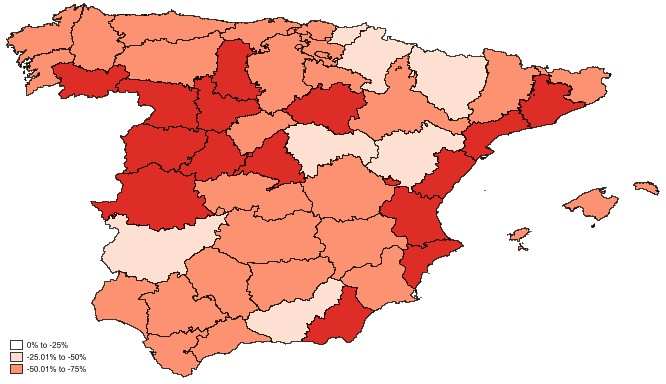
\includegraphics[width=.8\linewidth]{Figures/graph branches sin título.jpg}
  % \vspace{0.3em}

  % {\small\itshape Source: the authors.}
\end{figure}


\pagebreak
\clearpage




\begin{figure}%[htbp]
  \centering
 \caption{Evolution of population (2008 vs. 2019)}
 \caption*{\footnotesize This map displays the percentage change in population across Spanish provinces between 2008 and 2019. Darker blue shading indicates provinces with the largest population losses (over 15\% decline), while lighter shading represents more moderate changes (--5\% to 0\%). White areas indicate provinces with population growth or stability. The map reveals significant depopulation in interior provinces such as Teruel, Cuenca, Soria, and Zamora---territories often referred to as ``España vaciada'' (or \textsl{emptied Spain})---characterized by chronic depopulation, aging populations, and rural exodus. In contrast, urban centers such as Madrid and Barcelona, as well as coastal provinces, show population stability or modest growth during the study period, reflecting the concentration of economic opportunities and migration flows toward major metropolitan areas.}
  \label{fig:evolution_population}
  \vspace{10mm}
  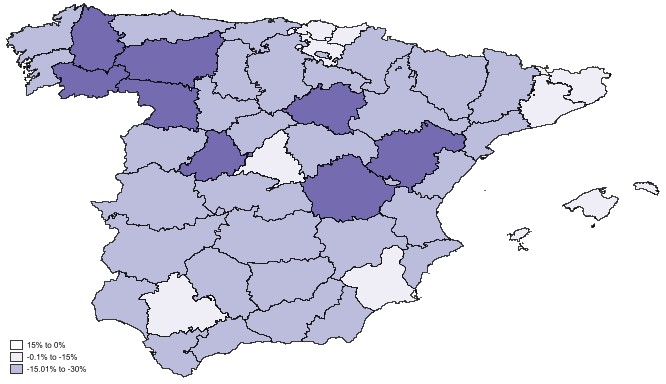
\includegraphics[width=.8\linewidth]{Figures/graph population sin título.jpg}
  % \vspace{0.3em}

  % {\small\itshape Source: the authors.}
\end{figure}


\pagebreak
\clearpage




\begin{figure}%[htbp]
  \centering
 \caption{Evolution of employment (2008 vs. 2019)}
 \caption*{\footnotesize This map displays the percentage change in employment (measured by registered employment contracts) across Spanish provinces between 2008 and 2019. Darker green shading indicates provinces with the largest employment gains (over 100\%), while lighter shading represents more moderate increases (0-25\%). The map shows considerable heterogeneity in employment dynamics across Spain. Several provinces experiencing significant population loss (see Figure \ref{fig:evolution_population}) paradoxically show substantial employment growth, suggesting a relative growth effect: fewer active workers but higher employment rates among the remaining population. Provinces such as Madrid and Barcelona, which had high employment levels before 2008, show lower relative growth rates despite strong absolute employment gains. The spatial pattern reflects the complex interplay between demographic decline, economic restructuring, and labor market dynamics during the post-crisis recovery period, with the services sector driving much of the observed employment growth.}
  \label{fig:evolution_employment}
  \vspace{10mm}
  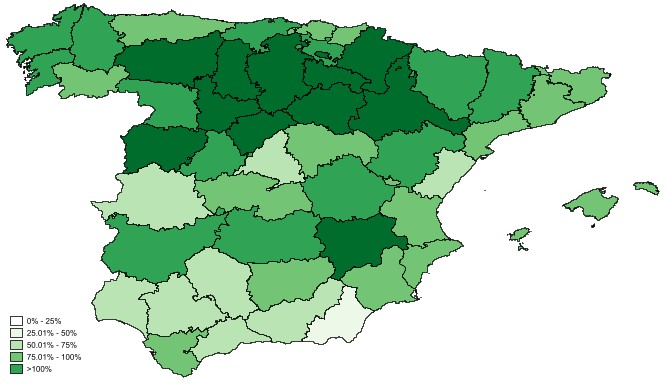
\includegraphics[width=.8\linewidth]{Figures/Graph Employment sin título.jpg}
  % \vspace{0.3em}

  % {\small\itshape Source: the authors.}
\end{figure}


\pagebreak
\clearpage




% \begin{figure}%[htbp]
%   \centering
%  \caption{Spanish NUTS-2 regions (\textsl{comunidades autónomas})}
%  \caption*{\footnotesize This map...}
%   \label{fig:map_ccaa}
%   \vspace{10mm}
%   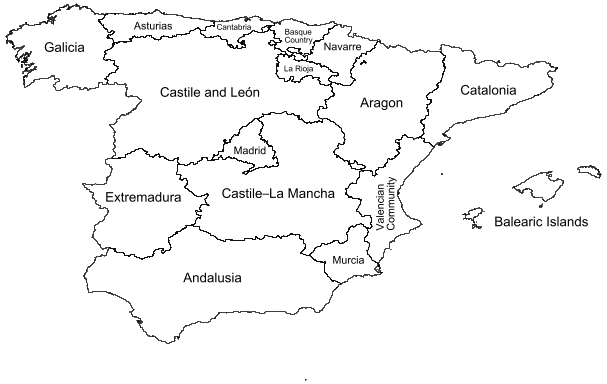
\includegraphics[width=.99\linewidth]{Figures/CCAA.jpg}
%   % \vspace{0.3em}

%   % {\small\itshape Source: the authors.}
% \end{figure}


\begin{figure}%[htbp]
  \centering
 \caption{Spanish NUTS-2 regions (\textsl{comunidades autónomas})}
 \caption*{\footnotesize This map displays the 16 Autonomous Communities (\textit{comunidades autónomas}) of peninsular Spain and the Balearic Islands included in the analysis. These NUTS-2 regions constitute the first level of sub-national administrative division and capture substantial heterogeneity in economic structure, demographic trends, and banking infrastructure. The regions with the largest number of municipalities in our sample are Castile and León (28.05\%), Catalonia (11.78\%), and Castile-La Mancha (11.47\%), while Murcia (0.56\%), the Balearic Islands (0.84\%), and Asturias (0.97\%) contribute the fewest. The Canary Islands are excluded from the analysis due to data unavailability. Our sample covers 8,014 municipalities, representing 98.84\% and 98.55\% of all registered municipalities in 2008 and 2019, respectively.}
  \label{fig:map_ccaa}
  \vspace{10mm}
  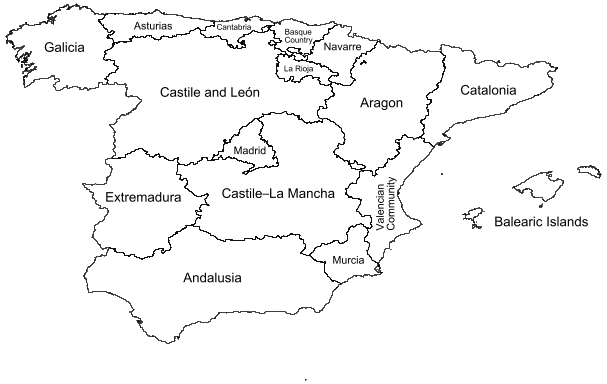
\includegraphics[width=.99\linewidth]{Figures/CCAA.jpg}
  % \vspace{0.3em}
  % {\small\itshape Source: the authors.}
\end{figure}



\pagebreak
\clearpage

% \begin{figure}%[htbp]
%   \centering
%  \caption{Spanish NUTS-3 provinces (\textsl{provincias})}
%  \caption*{\footnotesize This map...}
%   \label{fig:map_provinces}
%   \vspace{10mm}
%   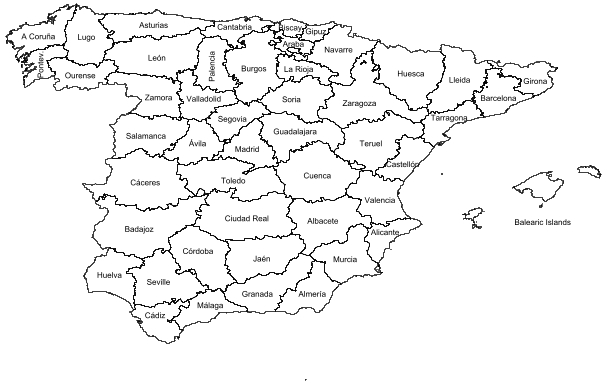
\includegraphics[width=.99\linewidth]{Figures/Provincias.jpg}
%   % \vspace{0.3em}

%   % {\small\itshape Source: the authors.}
% \end{figure}


\begin{figure}%[htbp]
  \centering
 \caption{Spanish NUTS-3 provinces (\textsl{provincias})}
 \caption*{\footnotesize This map displays the 48 provinces (\textit{provincias}) of peninsular Spain and the Balearic Islands included in the analysis, out of a total of 50 Spanish provinces (Ceuta and Melilla are autonomous cities). Provinces constitute the NUTS-3 level of administrative division and serve as the basis for the fixed effects included in our model. The provinces with the highest number of municipalities in the sample are Burgos (4.63\%), Salamanca (4.52\%), and Barcelona (3.88\%), while Cádiz (0.55\%), Murcia (0.56\%), and Álava (0.64\%) contribute the fewest. The two provinces belonging to the Canary Islands are excluded due to data unavailability. In 2008, nearly all provinces achieved full municipal representation, with only Girona (2 missing municipalities, 99.10\%), Biscay (1 missing, 99.11\%), and Zaragoza (1 missing, 99.66\%) falling slightly short. On average, the representation of municipalities across provinces was 99.96\% in 2008 and 99.51\% in 2019.}
  \label{fig:map_provinces}
  \vspace{10mm}
  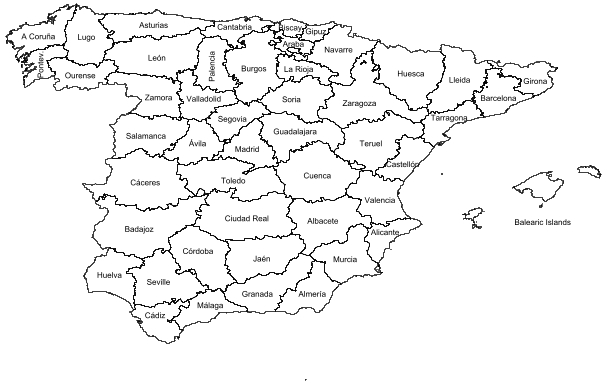
\includegraphics[width=.99\linewidth]{Figures/Provincias.jpg}
  % \vspace{0.3em}
  % {\small\itshape Source: the authors.}
\end{figure}


\pagebreak
\clearpage

% \begin{figure}%[htbp]
%   \centering
%  \caption{Spanish municipalities (LAU-2 level)}
%  \caption*{\footnotesize This map...}
%   \label{fig:map_municipalities}
%   \vspace{10mm}
%   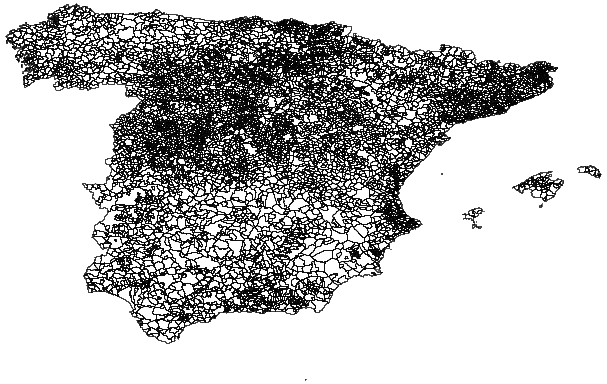
\includegraphics[width=.99\linewidth]{Figures/Municipios.jpg}
%   % \vspace{0.3em}

%   % {\small\itshape Source: the authors.}
% \end{figure}


\begin{figure}%[htbp]
  \centering
 \caption{Spanish municipalities (\textsl{municipios}), LAU-2 level}
 \caption*{\footnotesize This map displays the 8,014 municipalities (\textit{municipios}) included in the analysis, which constitute the primary unit of observation in our simultaneous equations model. Municipalities represent the finest level of local administrative division in Spain and exhibit a great deal of heterogeneity in terms of population size, economic activity, and access to banking services. In 2008, the average municipality in the sample had a population of 5,479 inhabitants, although the median was only 568, reflecting the highly skewed distribution of population across Spanish territory---with a large number of very small rural municipalities coexisting alongside a few major urban centres. The sample covers municipalities classified as urban, intermediate, and rural according to their degree of urbanisation, with rural municipalities serving as the reference category in our econometric specification. This granular level of analysis allows us to capture within-municipality dynamics, spatial spillovers from neighbouring municipalities, and the heterogeneous effects of employment and bank branch changes across different types of territories.}
  \label{fig:map_municipalities}
  \vspace{10mm}
  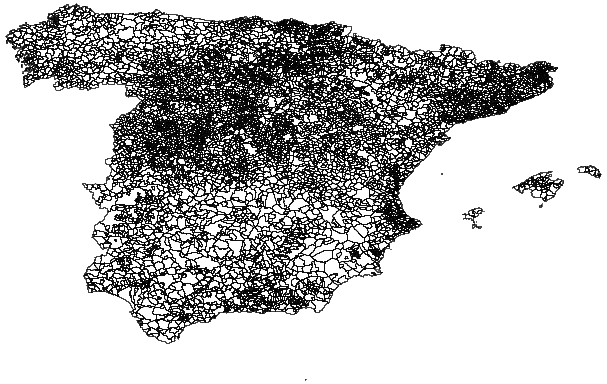
\includegraphics[width=.99\linewidth]{Figures/Municipios.jpg}
  % \vspace{0.3em}
  % {\small\itshape Source: the authors.}
\end{figure}





\end{document}









